%% CHAPTER 2 (probably)
%% MODELLING and DATA

\chapter{Data and Modelling} %with GEOS-Chem} % Main chapter title
\label{Model} %better reference name?
  
\section{Introduction}
  %Why use models?
  % Models
  
  In this thesis the word model is most often used to represent a chemical transport model (CTM), which simulates chemistry and chemical transport through the atmosphere.
  Models of the atmosphere can be used to improve measurements, estimate concentrations in regions not sampled, and allow predictions of atmospheric composition in the future.
  Models of ozone in the atmosphere are used broadly for international assessments of ozone related emissions and processes which involve ozone (such as radiation) \parencite{Young2018}.
  %\textcite{Young2018} summarise current global ozone modelling standards and the metrics and processes used to evaluate these models.
  Models can provide an estimate of trace gas concentrations without requiring measurements, however verification is required.
  
  
  In-situ measurements from campaigns or measurement stations can be used to examine what is happening at a particular (or several) location(s).
  These data are useful to determine how accurate models or estimates are - however the utility is limited to where the measurements have been made.
  In this thesis several campaigns are compared against model outputs.
  
  %Satellite usage and reduction of uncertainty
  Satellite datasets give us access to lots of data over large areas.
  However, satellite measurements can have high amounts of uncertainty due to instrument limitations.
  Many datapoints can be averaged in order to reduce uncertainty.
  In this thesis several satellite datasets are combined to provide biogenic HCHO amounts over Australia.
  In order to compare satellite data with other datasets, some work must be undertaken to avoid introducing bias \parencite[eg.][]{Palmer2001, Eskes2003, Marais2012, Lamsal2014}.
  
  In this chapter, modelled data are compared against both campaign measurements and satellite data in order to analyse Australia specific HCHO and isoprene sensitivities and to determine where the GEOS-Chem model needs the most improvement.
  Section \ref{Model:Datasets} lists and describes the campaign datasets, section \ref{Model:GC} describes the GEOS-Chem model, the creation and effects of filters are described in section \ref{Model:Filter}TODO: rest of section outlined.
  
  % MOVE: this is method not intro
   
  

\section{Datasets}
\label{Model:Datasets}

  %TODO: Combine these sections
  %\section{Campaigns}
  Here I will describe the various datasets I've used to analyse GEOS-Chem output.
  I will also give details on filtering and groupings which are undertaken when reading data, as each dataset has its own resolution.
  These datasets are used my thesis to determine isoprene emissions estimations in chapter \ref{BioIsop} and ozone transport extrapolations in chapter \ref{Ozone}.
  
  %TODO: Add all campaigns to the plot of locations
  Figure \ref{Model:Datasets:fig_locations} shows the locations of each of the campaigns I mention in this text.
  These took place over disparate times, and are in-situ measurements which require filtering and interpolation in order to compare against GEOS-Chem output which is averaged over a large horizontal space.
  
  \mypic{Figures/campaigns/campaign_locations.png}{Locations of Australian campaigns which are analysed within this thesis}{\label{Model:Datasets:fig_locations}}
  
  TODO: these summaries.
  
  \subsection{Daintree}
    Daintree summary (P. Nelson)
  
  % TODO: MUMBA summary
  \subsection{Marine and Urban MBA ? (MUMBA)}
    \label{Model:Datasets:MUMBA}
  
  \subsection{Sydney Particle Studies (SPS1, SPS2)}
    \label{Model:Datasets:SPS}
    Two VOC and other trace gas measurement campaigns took place at the Westmead Air Quality Station scientists from CSIRO, OEH, and ANSTO. 
    Stage 1 (SPS1) was from 5 February to 7 March in 2011, while stage 2 (SPS2) ranged from 16 April to 14 May 2012.
    
    Two instruments measured VOC concentrations: one was a Proton transfer reaction mass spectrometer (PTR-MS), the other a gas chromatographer (GC) with an equipped flame ionisation detector (FID).
    The PTR-MS uses chemical ionisation mass spectrometry and can quantify VOCs at high temporal resolution ($< 1$~s).
    It was calibrated several times per day against hcho, isoprene, $\alpha$-pinene, and several more VOCs. Further details can be found in \textcite{Dunne2012, Dunne2017} (TODO: Check papers).
    The output lists hourly averaged ppbv concentrations of trace gases based on the mass to charge ratio (m/z), which for isoprene is 69.
    It's possible that other chemicals (such as Furan, with the same m/z) interfered with this value, especially at low ambient isoprene concentrations and towards the end of autumn (SPS2) when wood fires usage starts to become frequent (TODO cite something).
    The GC-FID analysed samples collected in multi-absorbent tubes, with lower temporal resolution but no interferences. GC-FID data is averaged from 0500-1000~LT, and 1100-1900~LT. Further details for this method can be found in TODO: cite Min et al 2016.
    
    Figure \ref{Model:Datasets:SPS:fig_series} shows isoprene and formaldehyde over the course of these two campaigns, as well as the detection limits (dashed lines), as measured by PTR-MS. In order to compare with GEOS-Chem output a daily average and an overpass time (1200-1300 LT) average are both created from these data.
    In averaging, any measurements below the machine detection limit are set to half of the detection limit, as done in (TODO: doi:10.5194/acp-15-223-2015, 2015) which should minimise any introduced bias.
    
    \mypic{Figures/campaigns/SPS_Series.png}{
      SPS HCHO (yellow) and isoprene (green) time series, along with detection limits (dashed).
      SPS 1 (left) took place in late summer 2011, while SPS 2 (right) occurred during Autumn.
    }
    {\label{Model:Datasets:SPS:fig_series}}
    
    Figure \ref{Model:Datasets:SPS:fig_GC_comparison} shows GEOS-Chem output in the gridsquare containing Sydney overlaid on SPS measurement data.
    Superficially the comparison is not too bad between these two datasets, however GEOS-Chem output is daily averaged over 2x2.5\degr (latitude by longitude)
    The SPS data is point-source and taken during the daytime when isoprene is higher, so it is very likely that GEOS-Chem HCHO and isoprene output is in fact too high.
    
    \mypic{Figures/OMI_link/GC_vs_Campaigns_20050131-20050601.png}{Comparison between GEOS-Chem HCHO concentrations in the gridsquare containing Sydney for the duration of the SPS 1 and 2 campaigns}{\label{Model:Datasets:SPS:fig_GC_comparison}}
  
  \subsection{Satellite}
    \label{Model:Datasets:Aura}
    
    % Satellite data product levels
    Satellite data products are generally classed into several categories, level 0 through to level 3. Level 0 products are sensor counts and orbital swath data, level 1B data calibrates and geo-locates the level 0 data. 
    Level 2 products additionally have temporal, spatial, solar, and viewing geometry information, as well as quality flags.
    To create level 2 data slant column density is determined and then translated into vertical column density using an AMF calculated through radiative transfer models. 
    Level 3 data is a temporally aggregated version of the this, for instance monthly or yearly averages.
    
    % Aura satellite trace gas measurements
    One satellite is NASA's Earth Observing System's ``Aura'', which provides several useful datasets (products).
    Aura orbits the earth in a polar sun-synchronous pattern, circling the earth on a plane coincident with the sun and the poles.
    % omi instrument on board aura
    Aura houses the Ozone Monitoring Instrument (OMI), a near-UV/Visible Charged Coupled Device (CCD) spectrometer.
    From here on the word pixel is used to describe one data point retrieved by OMI, each pixel includes a latitude and longitude within OMI's data product.
    OMI measures several atmospheric trace gases, including NO$_2$, SO$_2$, BrO, HCHO, O$_3$, and aerosols.
    OMI measurements occur from right to left on a band covering 115$^{\circ}$, resulting in swaths of around 2600~km, with pixel sizes from 13x24~km$^2$ at nadir to 26x135~km$^2$ at the swath edges \parencite{Abad2015}.
    The swaths cover Earth daily, although half of these are at night time and contain no useful near-UV/Visible information.
    OMI spectra are used in several products used in this thesis, including OMNO2d, OMHCHO, and OMAERUVd.
    
    % Terra/Aqua satellite
    
    \subsubsection{OMNO2}
      \label{Model:Datasets:OMNO2d}
      NO$_2$ measured by OMI is used to check whether NO$_2$ is well represented by GEOS-Chem. 
      OMNO2d is a gridded daily level three product with good satellite pixels averaged into 0.25x0.25$^{\circ}$ horizontally resolved bins.
      An example figure from Jan 29, 2005 is shown in figure \ref{Model:Datasets:OMNO2d:fig_eg_omno2d}, while an average for 2005 (global) is shown in figure \ref{Model:Datasets:OMNO2d:fig_omno2d_2005}.
      
      \mypic{Figures/OMNO2d_2005m0129.png}{Example of NO$_2$ tropospheric columns taken from the OMNO2d product.}{\label{Model:Datasets:OMNO2d:fig_eg_omno2d}}
      
      \mypic{Figures/OMNO2d_avg2005.png}
        {Average 2005 tropospheric NO$_2$ from OMNO2d with pixels screened for $<30\%$ cloud cover.}
        {\label{Model:Datasets:OMNO2d:fig_omno2d_2005}}
      
      See section \ref{Model:Analysis:NOx} for the comparison between this product and GEOS-Chem calculations.
    
    \subsubsection{OMHCHO}
      \label{Model:Datasets:OMHCHO}
      
      % How omhcho is produced
      Atmospheric HCHO can be measured using Differential Optical Absorption Spectroscopy (DOAS), as long as trace gases with similar features near the same wavelength are accounted for.
      A DOAS fit determines the total column amount of a trace gas along the path that the instrument views.
      This uses the Beer-Lambert law where radiance is reduced as light travels through a medium.
      I use the NASA OMHCHOv003 data product \parencite{Abad2015}, with HCHO determined using the spectral window $328.5$~nm$ - 356.5$~nm. 
      The algorithm used is based on direct fitting of radiances, and accounts for competing absorbers, under-sampling, and Ring effects.
      An OMI radiance measurement over the remote Pacific ocean is used instead of an irradiance measurement.
      This means that the slant columns ($\Omega_S$) are actually the difference with respect to the radiance reference column ($\Omega_{S_0}$).
      The full method details for slant column retrieval by OMI are outlined in section \ref{SuppNotes:Satellite:OMI_BOAS}.
      Slant columns range from $\sim 4\times 10^{15} $ to $\sim 6 \times 10^{16}$~molec cm$^{-2}$, with uncertainties from 30\% (larger columns) to over 100\% (smaller columns) \parencite{Abad2015}.
      
      
      % What the swathes look like
      OMHCHO level two data includes 14-15 daily swaths of measurements provided by NASA.
      Each swath contains roughly $9 \times 10^4$ pixels, each of which contains various data including latitude, longitude vertical column HCHO, etc.
      The OMHCHO dataset has a quality flag which can be used to remove unlikely or poor satellite measurements.
      The states represented by this quality flag are shown in table \ref{Model:Datasets:OMHCHO:tab_qflag} which is taken from \textcite{Kurosu2014}.
      Filtering bad or missing measurement pixels is preformed prior to any other filtering, this includes the datapoints affected by the row anomaly.
      This anomaly (\url{http://projects.knmi.nl/omi/research/product/rowanomaly-background.php}) affects radiance data at particular viewing angles, corresponding to a row on the CCD detectors, and is dynamic over time.
      The slant columns affected are flagged and easy to remove before further processing.
      
      \begin{table}
        \caption{OMI quality flag values table from \textcite{Kurosu2014}}
        \begin{tabular}{  l  l  p{10cm} }
          \hline
          \textbf{Value} & \textbf{Classification} & \textbf{Rational} 
          \\ \hline
          0 & Good & Column value present and passes all quality checks; data may be used with confidence. 
          \\ \hline
          1 & Suspect & Caution advised because one or more of the following conditions are present: 
          \begin{itemize}
            \item Fit convergence flag is $<$ 300 but $>$ 0: Convergence at noise level
            \item Column $+ 2 \sigma$ uncertainty $<$ 0 $<$ Column $ + 3 \sigma $ uncertainty
            \item Absolute column value $>$ Maximum column amount (1e19 molec cm$^{-2}$)
          \end{itemize}
          \\ \hline
          2 & Bad & Avoid using as one of the following conditions are present: 
          \begin{itemize}
            \item Fit convergence flag is $<$ 0 : No convergence, abnormal termination
            \item Column $+ 3 \sigma$ uncertainty $<$ 0
          \end{itemize}
          \\ \hline
          $<0$ & Missing & No column values have been computed; entries are missing
          \\ \hline
        \end{tabular}
        \label{Model:Datasets:OMHCHO:tab_qflag}
      \end{table}
      
      % Where does cloud product come from? it removes around 30% of non-qa filtered data
      The cloud fraction with each pixel is provided with the OMHCHO dataset, however its source is the OMI cloud product, OMCLDO2.
      If greater than 40\% of a pixel measurement is cloudy (ie. cloud fraction $>0.4$) then the pixel is removed from subsequent analysis.
      This removes around 30\% of the pixels which remain after filtering out the bad or missing data.
      
      Each $\sim90$ minutes the AURA satellite sweeps over the sunny side of the planet, with OMI recording roughly 90~k pixels, of which around 50~k -- 80~k are classified as good.
      Each pixel contains several important pieces of data which are needed for recalculation of the HCHO vertical column: the total column of HCHO ($\Omega$\moleccm), cloud fraction, associated shape factor, AMF, geometric AMF, scattering weights and their vertical altitudes (hPa), viewing zenith angle, solar zenith angle, latitude, longitude, OMI sensor track, main data quality flag, cross track flag, and total column uncertainty.
      All of these data are needed in order to reconstruct the total vertical column using a modelled a priori shape factor rather than NASA's included a priori shape factor.
      
      Recalculated OMI formaldehyde columns are used as a basis for estimating isoprene emissions in Chapter \ref{BioIsop}.
    
    \subsubsection{OMAERUVd}
      \label{Model:Datasets:OMAERUVd}
      
      % smoke aaod outline
      Aerosols in the atmosphere can be seen through their affects on light. 
      Smoke and dust can be seen as an increase in AAOD (see section \ref{Model:Meas:DOAS}).
      This is due these particles scattering and absorbing UV radiation \parencite{Ahn2008}.
      
      
      %TODO: OMAERUVd brief description
      OMAERUVd (DOI: 10.5067/Aura/OMI/DATA3003) provides a useful dataset allowing us to filter gridsquares which may be smoke affected.
      OMI aerosol extinction and absorption optical depths (AOD, AAOD respectively) at three wavelengths (354, 388, and 500~nm), along with UV aerosol index (UVAI), are available publicly from Earthdata: \url{https://disc.gsfc.nasa.gov/datasets/OMAERUVd_V003/summary}.
      The OMAERUVd product is level three, gridded daily data, based on quality filtered level two swath pixels which are then gridded by averaging.
      The product is most sensitive to error in the form of subpixel scale cloud interference, so I select AAOD as the basis for my smoke filter as it is least affected by clouds \parencite{Ahn2008}.
      
      % How I read the AAOD
      Gridded smoke AAOD is read from OMAERUVd at 1x1\degr resolution daily, and mapped to finer resolution using the nearest value for each gridsquare.
      I use the AAOD at 500~nm wavelength, which is blocked by fire smoke plumes.
      This daily AAOD is used to mask fire smoke plume influence, by masking gridsquares with higher AAOD$>0.03$.
    
    \subsubsection{MOD14A1}
      \label{Model:Datasets:MOD14A1}
      Daily gridded fire counts compiled from Terra and Aqua satellite into 1x1~km$^2$ resolution.
      Using this product after binning into a lower resolution alows an active fire influence mask (see section \ref{Model:Filter:fire}.
      
      
  
  \subsection{Drought Index}
    The S Precipitation Evapotranspiration Index (SPEI) is a measure of drought using various parameters such as TODO. (\textcite{Wang2017}).
    SPEI will be compared against the difference between top-down estimated emissions and MEGAN bottom up estimated emissions. 
    This is used to determine whether there are biases in the MEGAN calculations due to the GEOS-Chem implementation ignoring soil moisture.
    It is downloaded from TODO and holds monthly averaged values at 0.5$^{\circ}$ horizontal resolution.
    When comparing against the emissions estimates this is interpolated linearly onto the same grid as that of GEOS-Chem output at 2x2.5$^{\circ}$.
    
  \subsection{NPI}
    
    One possible solution to anthropogenic filtering is the national pollution index (TODO:cite:\verb|http://www.npi.gov.au|) which contains industrial HCHO and NO$_X$ emissions from 2003 to 2014.
  
  % TODO: Move this section INTO GEOS-Chem section!!!
\section{GEOS-Chem}
  \label{Model:GC}

  \subsection{Outline}
    % Geos chem is a box model with chemistry and meteorology
    GEOS-Chem is an atomspheric chemical model (ACM), using a 3-D grid of boxes with transport driven by the GEOS meteorological model and chemistry calculated in each box independently. 
    Within each box chemistry, transport, and meteorology are simulated at 15 minute time steps.
    GEOS-Chem has a meteorological model coupled to a chemical model, which simulates the world in a three dimensional grid of connected boxes.
    
    % It uses GEOS, from GMAO
    GEOS-Chem is a well supported global, Eulerian CTM with a state of the science chemical mechanism, with transport driven by meteorological input from the Goddard Earth Observing System (GEOS) of the NASA Global Modeling and Assimilation Office (GMAO).
    GEOS-Chem simulates more than 100 chemical species from the earth's surface up to the edge of space (0.01~hPa) and can be used in combination with remote and in-situ sensing data to give a verifiable estimate of atmospheric gases and aerosols.
    It was developed, and is maintained, by Harvard University staff as well as users and researchers worldwide.
    In this thesis I use version 10.01 of GEOS-Chem, which simulates and records up to 66 chemical species (tracers) in the standard run, at 2 by 2.5$^{\circ}$ horizontal resolution, with 47 levels up to the top of the atmosphere (TOA at 0.01~hPa). 
    
    % This thesis uses 10.01, geos5, megan
    Global CTMs are often run using one or several emission models (or the output from them) to determine boundary conditions for many gridboxes.
    Some of the inventories are described here.
    Meteorological fields are taken from NASA's GEOS-5 dataset (0.5$^{\circ}$ x 0.666$^{\circ}$) \parencite{Chen2009}, which exists up to April, 2013.
    GEOS-5 meteorological fields are used as the boundary conditions driving transport.
    % Emissions models used for boundary conditions
    Fire emissions come from the GFED4 product \parencite{Giglio2013}. 
    Anthropogenic VOC emissions come from the EDGAR inventory, while biogenic VOC emissions are simulated using the MEGAN model.
    MEGAN is used to determine biogenic emissions for our default GEOS-Chem simulation, described in more detail in section TODO.
    The estimated biogenic VOC emissions are important for accurately simulating chemistry within models, as discussed in Section \ref{LR:Atmos:Chem}.
    
  
  \subsection{Running GEOS-Chem (before isop?)}
    \label{Model:GC:running}
    \subsubsection{Installation and requirements}
      GEOS-Chem instructions for download, compilation, and running can be found in the user guide provided by Harvard: \url{http://acmg.seas.harvard.edu/geos/doc/man/}.
      In order to build and run GEOS-Chem a high-speed computing system is optimal, as globally gridded chemical calculations can take a long time to perform.
      I installed GEOS-Chem onto a suitably configured workspace on the National Computational Infrastructure (NCI, \url{http://nci.org.au/}). 
      This workspace included access to compilers and libraries which are needed to build the Fortran based GEOS-Chem source code, and IDL, Python, and various editors and scripting languages to read, run, edit, and analyse both GEOS-Chem and its output.
      
      After downloading GEOS-Chem, the code can be compiled with different options for resolution and chemical mechanisms.
  
  \subsection{GEOS-Chem isoprene modelling}
    \label{Model:GC:Isop}

    \subsubsection{Outline}
      The isoprene reactions simulated by GEOS-Chem were originally based on \textcite{Horowitz1998}.
      This involved simulating NO$_X$, O$_3$, and NMHC chemistry in the troposphere at continental scale in three dimensions, with detailed NMHC chemistry with isoprene reactions and products.
      The mechanism was subsequently updated by \textcite{Mao2013}, who change the isoprene nitrates yields and add products based on current understanding as laid out in \textcite{Paulot2009a,Paulot2009b}.
      Further mechanistic properties, like isomerisation rates, are based on results from four publications: cite{Crounse2011,Crounse2012,Peeters2010,Peeters2011}.
      (TODO: check abstracts Peeters papers).
      
      \textcite{Crounse2011} examines the isomerisations associated with the oxidation of isoprene to six different isomers of ISOPOO formed in the presence of oxygen through $ISOP + OH \to ISOPOO$.
      They determine rates and uncertainties involved in these reactions, and study the rate of formation of C$_5$-hydroperoxyaldehydes (HPALDs) by isomerisation.
      Methacrolein (MACR) is one of the products of isoprene oxidation.
      Prior to 2012 MACR oxidation chamber studies were performed in high NO or HO$_2$ concentrations, giving peroxy lifetimes of less than 0.1~s \parencite{Crounse2012}.
      In most environments this is not the case, GEOS-Chem uses MACR production rates for different NO concentrations and peroxy radical lifetimes determined by \textcite{Crounse2012}.
      Additionally, photolysis of photolabile peroxy-acid-aldehydes creates OH and improved model aggreement with continental observations.
      photolysis of hydroperoxy-methyl-butenals (HPALDs, produced by isoprene isomerisation) regenerate OH levels in areas with high isoprene emissions \parencite{Peeters2010}.
      OH and HPALD interactions are central to maintaining the OH levels in pristine and moderately polluted environments, which makes isoprene both a source and a sink of OH \parencite{Peeters2010,Taraborrelli2012}.
      
      Formation of isoprene nitrates have an effect on ozone levels through NO$_X$ sequestration, and the yields and destinies of these nitrates is analysed in \textcite{Paulot2009a}.
      In a chamber with clean air and high NO concentrations, isoprene photooxidation is initially driven by OH addition, followed by NO$_X$ chemistry (150~min - 600~min), and finally HO$_X$ dominated chemistry.
      GEOS-Chem uses these the yields of various positional isomers of isoprene nitrates, and pathways of their oxidation products, and reactions within its suite of chemical mechanisms determined by \textcite{Paulot2009a,Mao2013}.
      %They use anion chemical ionization mass spectrometry (CIMS) to determine products of isoprene photooxidation.
      
      In low NO$_X$ conditions, isoprene oxidises to yield 70\% hydroxyhydroperoxides (ISOPOOH), which then oxidises to create dihydroxyperoxides (IEPOX) with OH recycling maintaining the OH levels in the atmosphere \parencite{Paulot2009b}.
      In older models isoprene produced ISOPOOH which then titrated OH, however, the loss of OH has not been seen in measurements \parencite{Paulot2009b,Mao2013}.
      The isoprene mechanism in GEOS-Chem has been updated to include OH regeneration from oxidation of epoxydiols and slow isomerisation of ISOPO$_2$ \parencite{Mao2013}.
      
      ISOPN can be oxidised (by OH) to form nitrated organic products \parencite{Paulot2009a}.
      In low NO$_X$ ISOPOO reacts with HO$_2$ (producing hydroxy hydroperoxides, ISOPOOH), RO$_2$ (producing mainly MACR, MVK, and HCHO), or isomerises (1,5-H shift producing MACR, MVK, HCHO, or 1,6-H shift producing hydroperoxyenals HPALDs). 
      ISOPOOH can be oxidised (by OH) to produce epoxydiols (IEPOX), precursors to SOA \parencite{Paulot2009b}. 
      HPALDs can photolyse to regenrate OH and small VOCs \parencite{Crounse2011,Wolfe2012, Peeters2014} TODO: Check out crounse2011.
      See section \ref{LR:VOCs:IsopCascade} for more information.
      
      Under high NO$_X$ conditions, isoprene undergoes OH addition at the 1 and 4 positions, becoming $\beta$ (71\%) or $\delta$ (29\%) hydroxyl peroxy radicals (ISOPO$_2$). 
      The $\beta$-hydroxyl reacts with NO$_X$ and produces HCHO (66\%), methylvinylketone (40\%) (MVK), methacrolein (26\%), and $\beta$-hydroxyl nitrates (6.7\%) (ISOPNB).
      The $\delta$-hydroxyl reacts with NO to form $\delta$-hydroxyl nitrates (24\%) (ISOPND), and ISOPNB (6.7\%).
      ISOPNB and ISOPND yield first generation isoprene at 4.7\% and 7\% respectively.
      
      Under low NO$_X$ conditions, ISOPO$_2$ may react with HO$_2$ to form ISOPOOH.
      In this case there is also production of HCHO (4.7\%), MVK(7.3\%), and MACR (12\%).
      As stated in earlier; most ISOPOOH will form IEPOX (epoxydiols) after reacting with OH and lead to OH regeneration.
      The other mechanism in low NO$_X$ environments is unimolecular isomerisation of ISOPO$_2$.
      This leads to production of hydroperoxyaldehydes (HPALDS), which generally photolyse and have an OH yield of 100\%.
      \textcite{Mao2013} show that a lower (factor of 50) rate constant for ISOPO$_2$ isomerisation leads to better organic nitrate aggreements with ICARTT. 
      
      This update leads to more accurate modelling of OH concentrations, especially in low NO$_X$ conditions common in remote forests.
      Prior to \textcite{Mao2012}, measurements of OH in high VOC regions may have been up to double the real atmospheric OH levels, due to formation of OH inside the instrument.
      \textcite{Mao2012} examine an upgraded method of measurement, and compare these against a regional atmospheric chemistry model (RACM2), with the OH recycling updates from \textcite{Paulot2009b} as discussed in prior paragraphs.
      
      The updates to isoprene chemistry by \textcite{Mao2013}, and those shown in \textcite{Crounse2011,Crounse2012} are the last before version 11.
      The full current mechanism is described online at \url{http://wiki.seas.harvard.edu/geos-chem/index.php/New_isoprene_scheme}.
  
  \subsection{Chemical Mechanisms}
    \label{Model:GC:Mechanisms}
    Chemical reactions are turned into systems of differential equations (DEs) to be solved by the CPU for each gridbox in GEOS-Chem.
    A chemical mechanisms is the name for a closed system of chemical reactions and the rates of each reaction.
    Simplifications are required due to the massive amount of reactions which occur in the atmosphere, and the coupled and stiff nature of these reactions which serve to slow down computation of the solutions TODO: ref Brasseur Jacob book.
    
    
    
    Some of the important ones involving isoprene are copied here, including reaction rates in the form $ k = A \exp{-ER/T} $.
    The full list of chemical reactions can be found online at TODO: find list
    
    \begin{align} \begin{split}
    \label{Model:GC:Mechanisms:eqn_mechanisms}
    \ce{
      RIO2 + NO ->[2.7*10^{-12} \exp{350/T}] & .883NO2 + .783HO2 + .66CH2O \\
      & + .4MVK + .26MACR + .07ISOPND \\
      & + .123HC5 + .1DIBOO \\
      RIO2 ->[4.07*10^{8} \exp{-7694/T}] & 2HO2 + CH2O + .5MGLY + .5GLYC \\
      & + .5GLYX + .5HAC + OH
    }
    %     % k1=2.7*10^{-12} \exp{350/T}
    %     % k2=4.07*10^{8} \exp{-7694/T}
    %      
    \end{split} \end{align}
  
  
  \subsection{Emissions from MEGAN}
    \label{Model:GC:Isop:MEGAN}

    MEGAN is a global model with resolution of around 1~km, and is used to generate the BVOC emissions used in various global chemistry models such as GEOS-Chem.
    MEGAN uses leaf area index, global meteorological data, and plant functional types (PFTs) to simulate terrestrial isoprene emissions.
    The model includes global measurements of leaf area index, plant functional type, and photosynthetic photon flux density, from remote sensing databases \parencite{Kefauver2014}.
    The various PFTs are used to generate emission factors which represent quantities of a compound released to the atmosphere through an associated activity.
    For example, an emission factor for isoprene within a forest would include the requirement of sunshine and suitable temperature.
    The schematic for MEGAN, taken from \textcite{Megan_Website}, is shown in figure \ref{Models:GC:Isop:MEGAN:fig_megan_schematic}
    
    \begin{figure}[!htbp]
      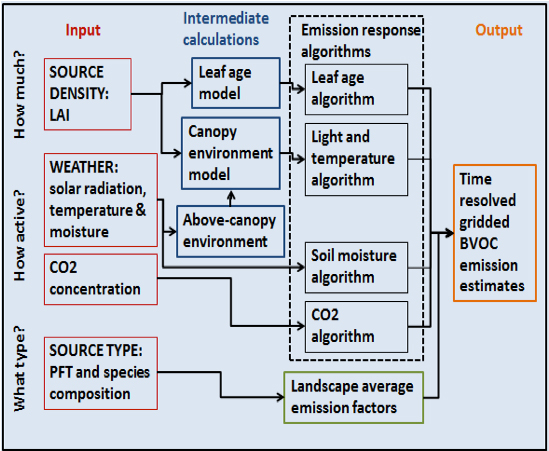
\includegraphics[width=\textwidth]{Figures/MEGANmodel_img.jpg}
      \caption{MEGAN schematic, copied from \textcite{Megan_Website}}
      \label{Models:GC:Isop:MEGAN:fig_megan_schematic}
    \end{figure}
    
    GEOS-Chem V10.01 uses MEGAN V2.1 with biogenic emissions from \textcite{Guenther2012}.
    It computes some emissions using predefined EF maps from MEGAN source code, and others using PFT maps and associated EFs.
    MEGAN ``is a modelling framework for estimating fluxes of biogenic compounds between terrestrial ecosystems and the atmosphere to account for the major known processes controlling biogenic emissions.'' \parencite{Guenther2012}.
    It allows parameterisation of various BVOC emissions, with descriptions given in \textcite{Guenther2012}.
    Instructions to run version 2.1 are available at \url{http://lar.wsu.edu/megan/docs/MEGAN2.1_User_GuideWSU.pdf}, and a version using the Community Land Model (CLM) is available at \url{http://www.cesm.ucar.edu}.
    It uses meteorological fields from the Weather Research and Forecasting (WRF) modelling system.
    Version 2.1 (updated from 2.0 \parencite{Guenther2006}) includes 147 species, in 19 BVOC classes, which can be lumped together to provide appropriate output for mechanisms in various chemical models.
    
    MEGAN was developed as a replacement for two earlier canopy-environment emission models (BIES and GEIA), and initially included a simple canopy radiative transfer model, which parameterised sun-lit and shaded conditions through a canopy.
    Early models didn't account for abiotic stresses, such as drought, prior rainfall and development processes. These stresses influenced species-specific emissions by more than an order of magnitude \parencite{Niinemets1999}.
    Isoprene emissions were based on temperature, leaf area, and light, but have since been updated to include leaf age activity \parencite{Guenther2000}, and a leaf energy balance model \parencite{Guenther2006} in MEGANv2.0.
    This update included a parameter for soil moisture, to account for drought conditions, however this parameter is currently (as of version 2.1) not applied to isoprene \parencite{Sindelarova2014}.
    Soil moisture effects on isoprene emission are very important, and can drastically affect estimates.
  
  \subsection{Rescaling NOx}
  
    NO$_X$ concentrations affect HCHO yield, isoprene lifetimes, and other things due to affects on the atmospheres oxidative capacity.
    This means that if the model is poorly simulating NO$_X$, isoprene to HCHO yield and transport (see \ref{BioIsop:Methods:Smearing}) may be poorly estimated.
    In order to determine if rescaling the NO emissions over Australia is necessary in GEOS-Chem, I looked at modelled NO$_2$ amounts compared to satellite data for most of 2005.
    
    % Geos chem vs tropno2 from omno2d
    Simulated GEOS-Chem tropospheric NO$_2$ columns averaged from 1300-1400~LT are compared against OMNO2d data (Sec. \ref{Model:Datasets:OMNO2d}). 
    Figure \ref{Model:Analysis:NOx:fig_GC_vs_OMNO2d_summer_2005} shows the direct comparison between these datasets averaged over the month of January, 2005.
    It's clear that the OMNO2d product can pick out Sydney and Melbourne as NO$_2$ hotspots, which are underestimated by GEOS-Chem due to averaging over the 2x2.5\degr horizontal resolution.
    Over much of the country GEOS-Chem overestimates NO$_2$ by 10-60\%, except in NA and northern Queensland where up to 50\% underestimation occurs.
    The correlation between the bias (GEOS-Chem - OMNO2d) with anthropogenic and soil emissions is shown in the bottom rows.
    The comparison for January and February of 2005 in Figure \ref{Model:Analysis:NOx:fig_GC_vs_OMNO2d_summer_2005}, and winter (JJA) of 2005 in in Figure \ref{Model:Analysis:NOx:fig_GC_vs_OMNO2d_summer_2005}.
    The poor correlations for anthropogenic NO suggest that blanket alterations over Australia would not lead to improved NO$_2$ fit. 
    
    \begin{figure}
      % Figure from GC_tests.py GC_vs_OMNO2d, then modified in paint
      % Summer correlation
      \includegraphics[width=\textwidth]{Figures/OMI_link/GC/GC_vs_OMNO2_AUS_20050101-20050228.png}
      \caption{%
        Row 1 shows the tropospheric columns in molec cm$^{-2}$, GEOS-Chem, OMNO2d, and OMNO2d averaged onto the lower resolution of GEOS-Chem from left to right.
        Row 2 shows the correlations of GEOS-Chem (X axes) between daily anthropogenic emissions, and mid-day OMNO2d columns.
        Row 3 shows the differences with OMNO2d columns averaged into the lower resolution of GEOS-Chem.
      }
      \label{Model:Analysis:NOx:fig_GC_vs_OMNO2d_summer_2005}
    \end{figure}
    
    \begin{figure}
      % Figure from GC_tests.py GC_vs_OMNO2d, then modified in paint
      % Winter correlation
      \includegraphics[width=\textwidth]{Figures/OMI_link/GC/GC_vs_OMNO2_AUS_20050101-20050228.png}
      \caption{%
        Row 1 shows the tropospheric columns in molec cm$^{-2}$, GEOS-Chem, OMNO2d, and OMNO2d averaged onto the lower resolution of GEOS-Chem from left to right.
        Row 2 shows the correlations of GEOS-Chem (X axes) between daily anthropogenic emissions, and mid-day OMNO2d columns.
        Row 3 shows the differences with OMNO2d columns averaged into the lower resolution of GEOS-Chem.
      }
      \label{Model:Analysis:NOx:fig_GC_vs_OMNO2d_winter_2005}
    \end{figure}
    
    This comparison is expanded, including a comparison against modelled emissions, and repeated for autumn (MAM), winter (JJA), and spring (SON) in figures \ref{Model:Analysis:NOx:fig_GC_vs_OMI_anthro_Sum} to \ref{Model:Analysis:NOx:fig_GC_vs_OMI_soil_Spr}.
    These show an analysis of GEOS-Chem NO emissions and their correlations with the bias between GEOS-Chem NO$_2$ mid-day columns and the OMNO2d product, averaged over each season in 2005.
    The scatter plots have one datapoint for each land square over Australia.
    
    The correlation between model and satellite NO$_2$ columns is OK throughout the year over Australia, with some overestimation in the north during non-summer months.
    There is also slight underestimation over Sydney and Melbourne throughout the year.
    Figures \ref{Model:Analysis:NOx:fig_GC_vs_OMI_anthro_Sum} to \ref{Model:Analysis:NOx:fig_GC_vs_OMI_soil_Spr} show that the visible biases are not over Australia are not driven by modelled emissions of NO.
    While the correlation between column NO$_2$ and emitted NO is clear, emissions do not appear to bias the model in either direction away from the satellite data.
    
    % Figures from GC_tests.py GCe_vs_OMNO2d
    \mypic{Figures/OMI_link/GC/GCanthro_vs_OMNO2_AUS_20050101-20050228.png}
    {
      Top row (left to right): GEOS-Chem NO$_2$ mid-day tropospheric columns, OMNO2d NO$_2$ columns, modelled anthropogenic NO emissions. 
      Second row: absolute and relative difference between GEOS-Chem and OMI NO$_2$ data, and the correlation.
      Third row: correlation between GEOS-Chem tropospheric column NO$_2$ and emitted NO, then between the model-satellite bias and the emissions.
      All correlation plots are coloured by emission rates.
    }
    {\label{Model:Analysis:NOx:fig_GC_vs_OMI_anthro_Sum}}
    
    \mypic{Figures/OMI_link/GC/GCanthro_vs_OMNO2_AUS_20050301-20050531.png}
    {As figure \ref{Model:Analysis:NOx:fig_GC_vs_OMI_anthro_Sum}, for Autumn 2005.}
    {\label{Model:Analysis:NOx:fig_GC_vs_OMI_anthro_Aut}}
    
    \mypic{Figures/OMI_link/GC/GCanthro_vs_OMNO2_AUS_20050601-20050831.png}
    {As figure \ref{Model:Analysis:NOx:fig_GC_vs_OMI_anthro_Sum}, for Winter 2005.}
    {\label{Model:Analysis:NOx:fig_GC_vs_OMI_anthro_Win}}
    
    \mypic{Figures/OMI_link/GC/GCanthro_vs_OMNO2_AUS_20050901-20051130.png}
    {As figure \ref{Model:Analysis:NOx:fig_GC_vs_OMI_anthro_Sum}, for Spring 2005.}
    {\label{Model:Analysis:NOx:fig_GC_vs_OMI_anthro_Spr}}
    
    % Soil pictures
    \mypic{Figures/OMI_link/GC/GCsoil_vs_OMNO2_AUS_20050101-20050228.png}
    {As figure \ref{Model:Analysis:NOx:fig_GC_vs_OMI_anthro_Sum}, except anthropogenic NO emissions are replaced by soil NO emissions.}
    {\label{Model:Analysis:NOx:fig_GC_vs_OMI_soil_Sum}}
    
    \mypic{Figures/OMI_link/GC/GCsoil_vs_OMNO2_AUS_20050301-20050531.png}
    {As figure \ref{Model:Analysis:NOx:fig_GC_vs_OMI_anthro_Sum}, for Autumn 2005, with soil NO emissions replacing anthropogenic NO emissions.}
    {\label{Model:Analysis:NOx:fig_GC_vs_OMI_soil_Aut}}
    
    \mypic{Figures/OMI_link/GC/GCanthro_vs_OMNO2_AUS_20050601-20050831.png}
    {As figure \ref{Model:Analysis:NOx:fig_GC_vs_OMI_anthro_Sum}, for Winter 2005, with soil NO emissions replacing anthropogenic NO emissions.}
    {\label{Model:Analysis:NOx:fig_GC_vs_OMI_soil_Win}}
    
    \mypic{Figures/OMI_link/GC/GCanthro_vs_OMNO2_AUS_20050901-20051130.png}
    {As figure \ref{Model:Analysis:NOx:fig_GC_vs_OMI_anthro_Sum}, for Spring 2005, with soil NO emissions replacing anthropogenic NO emissions.}
    {\label{Model:Analysis:NOx:fig_GC_vs_OMI_soil_Spr}}
    
    The conclusion drawn is that modelled anthropogenic and soil NO emissions do not show sufficient evidence of biasing GEOS-Chem NO$_2$ columns away from satellite measurements over Australia.
    For this reason modelled NO emissions are not scaled in model runs in this thesis.
  
  \subsection{GEOS-Chem simulations}
    \label{Model:GC:runs}
    
    GEOS-Chem is run four independent times in this thesis, with different outputs from each simulation used to determine specific information. 
    
    Output for an area averaged over 1300 - 1400 local time is saved for comparison and recalculation with satellite overpass records.
    These averages are used to calculate both the GEOS-Chem based AMF, and the modelled background HCHO over the remote pacific which is used in the reference sector correction for OMI column retrievals (see section \ref{Model:omiRecalc:RSC}).
    They are also used to determine isoprene to HCHO yield, after removing days with high biomass burning emissions.

    TODO: Go through work process and clarify these items
    Run descriptions and their outputs are listed here, with outputs described in more detail in section :
    \begin{enumerate}
      \item UCX 
      \begin{enumerate}
        \item Satellite output (1300-1400LT)
        \item Create shape factors for AMF recalculation in OMI
        \item This run was initially used to determine if the stratospheric chemistry had much influence over tropospheric isoprene or HCHO concentrations.
      \end{enumerate}
      
      \item Tropchem (standard)
      \begin{enumerate}
        \item satellite output, daily tracer averages
        \item Recreate the AMFs for OMI when running code from Dr. Paul Palmer, modified by Dr. Luke Surl.
        \item Combined with an identical run where isoprene emissions are halved in order to determine smearing.
        \item TODO: Compare total yearly isoprene emissions before and after new estimate.
      \end{enumerate}
      
      \item Tropchem(isoprene emissions halved)
      \begin{enumerate}
        \item In GEOS-Chem the isoprene emissions can be globally multiplied by a constant factor.
        \item An estimate of modelled HCHO sensitivity to isoprene emissions and transport (smearing) can be determined.
        \item Smearing is determined by running the model with the biogenic isoprene emissions halved while other parameters remain unchanged.
      \end{enumerate}
      
      \item Tropchem(biogenic emissions only, all other inventories turned off)
      \begin{enumerate}
        \item Satellite output, hourly biogenic emissions from MEGAN
        \item The output from this simulation is used to determine the biogenic yield from isoprene to HCHO over Australia, described in section \ref{BioIsop:Methods}.
        \item TODO: compared to run with updated emissions
      \end{enumerate}
      
    \end{enumerate}
    NB: for non-UCX runs, satellite output was modified to include tropopause height

      
      % TODO: layout reasons why isoprene differs between runs
      %    In GeosCore/fast_jx_mod.F:
      %      strat aerosols are scaled somehow at line 2922, looks like it affects SSA.
      %      line 4138: comment says ozone calculated online.
      %	  TOMS/SBUV O3 are read by toms_mod.f, passed to FAST-J routine ``set_prof.f''. in UCX the stratospheric O3 is calculated online
      %    In GeosCore/calcrate.F:
      %      line 1489 comment says rates are limited to prevent solver failure
      %	if lifetime of A is below PSCMINLIFE, limit reaction rate to yield the specified lifetimedepletion
      %      Line 1724
      %        ! SPECIAL TREATMENT FOR O3+hv -> OH+OH (trop-only simulation)
      %        !                    or O3+hv -> O+O2  (UCX simulation)
      %      line 1752:
      %      #if defined( UCX )
      %        IF ( NKO3PPHOT(NCS) > 0 ) THEN
      %          PHOTVAL_2 = NKO3PPHOT(NCS) - NRATES(NCS)
      %          NKN_2     = NKNPHOTRT(PHOTVAL_2,NCS)
      %        ENDIF
      %      #endif
      %      line 1771:
      %        comment: change rate of O(1D) + N2 to 3.1e-11 at 298K (from 2.6e-11)...
      %        if not defined UCX:
      %	  RO1Dp1H2O, RO1Dp1H2, RO1D, (and maybe 2 RRates) are changed.
      
    \subsubsection{Run comparisons}
  
      There are many options available when running GEOS-Chem depending on the desired chemistry, resolution, meteorology, and boundary conditions.
      Here we compare the model output with and without enabling the Universal tropospheric-stratospheric Chemistry eXtension (UCX).
      %From version 11 of GEOS-Chem, the UCX mechanism is enabled by default.
      Both runs use 2$^{\circ}$ latitude by 2.5$^{\circ}$ longitude, however the UCX mechanism is run with 72 vertical levels from the surface to the top of the atmosphere (TOA$\sim$0.1~hPa), while the standard (tropchem) run uses 47 levels.
      The extra vertical levels are added in the stratosphere, providing finer vertical resolution from around 70~hPa to the top of the atmosphere.
      For both runs the inpup parameters such as MEGAN emissions and GEOS-5 meteorological fields are identical.
      
      GEOS-Chem output of HCHO does not differ much between runs with or without the Unified Chemistry eXchange (UCX).
      Figure \ref{Model:GC:running:fig_UCXvsTrop_HCHO} shows an example of surface HCHO amounts with and without UCX turned on.
      The differences do not exceed 3\% over Australia for the averaged month of January, 2005.
      
      \begin{figure}%[!htbp] % TODO: remove 'rerun' plot, use normal and delete rerun thingy so it's not confusing later.
        % These figures created in GC_test.py -> TODO:
        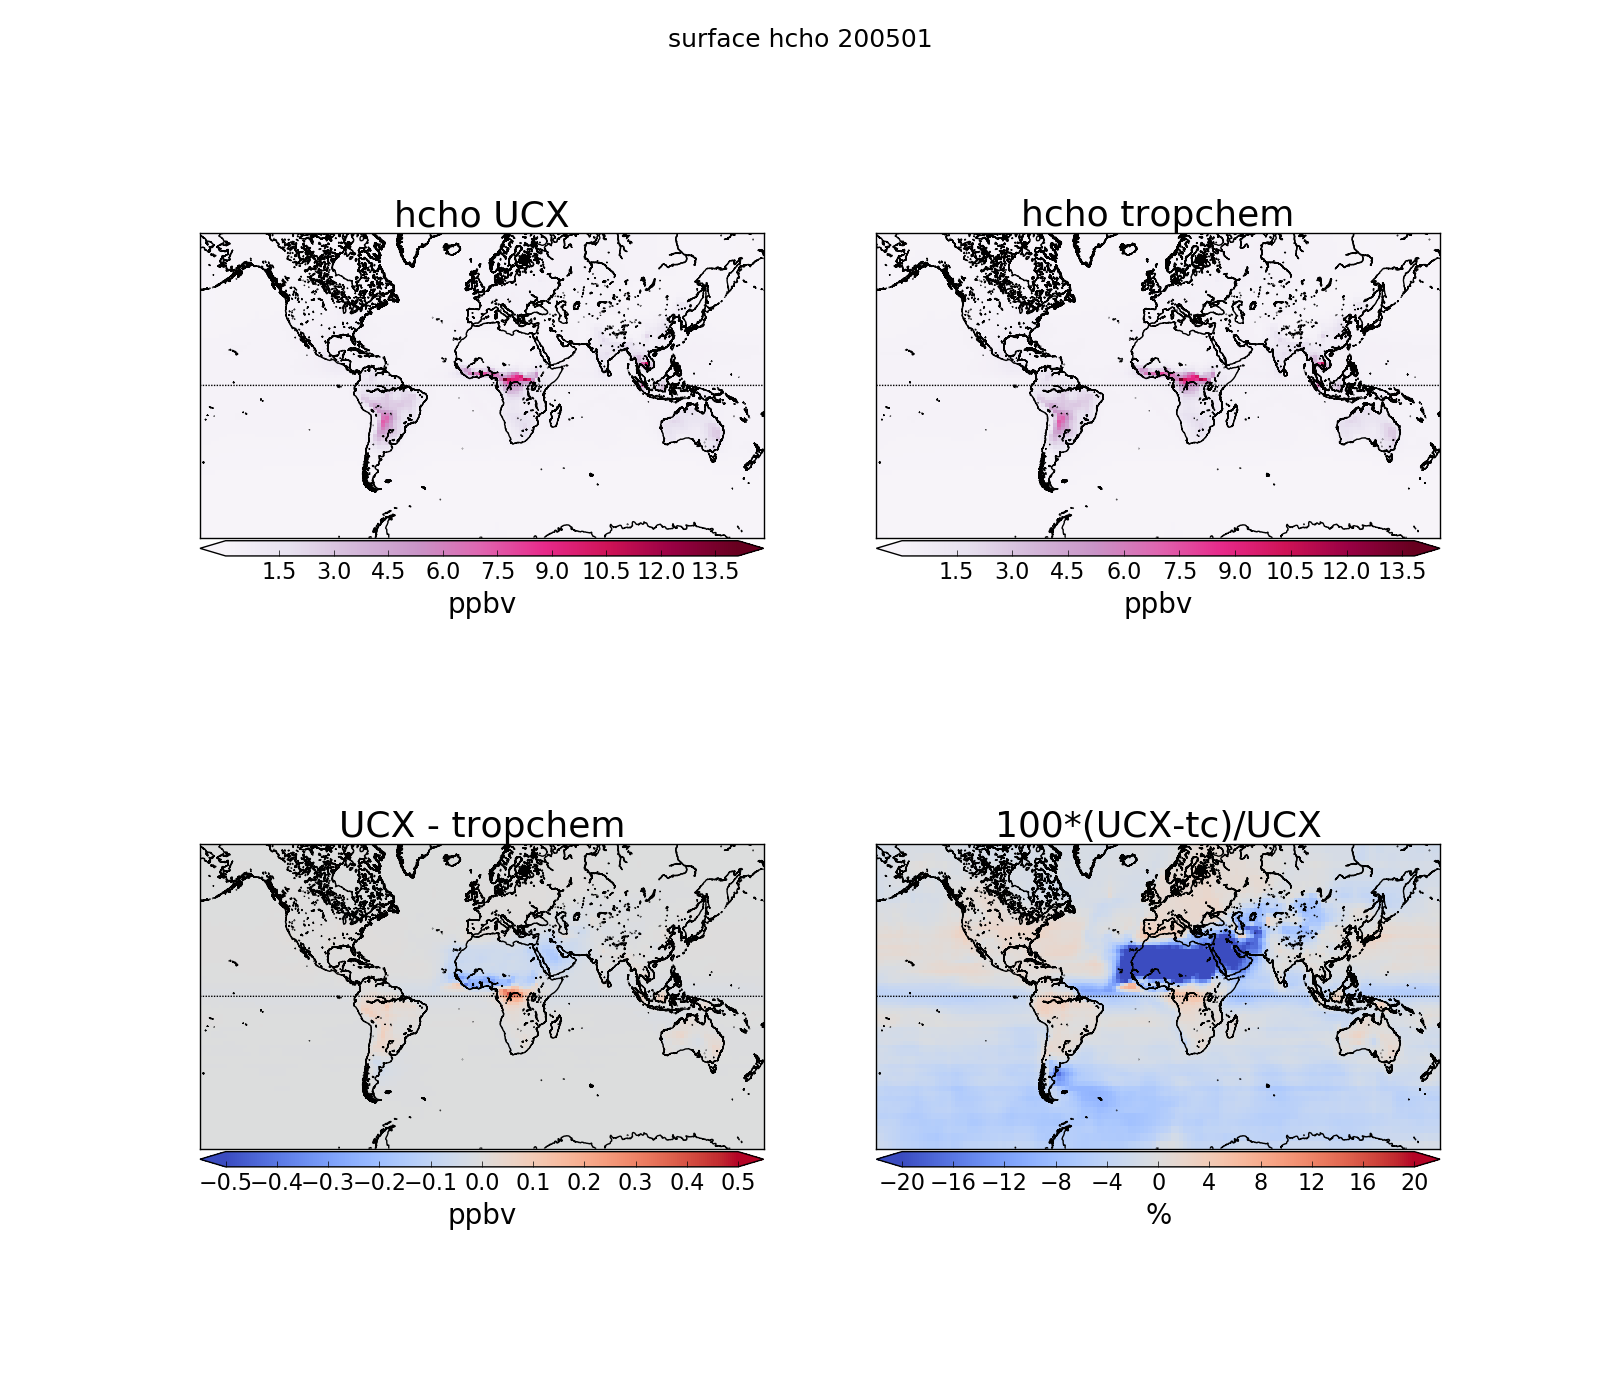
\includegraphics[width=\textwidth]{Figures/OMI_link/GC/UCX_vs_trp_glob_200501_hcho_rerun.png}
        \caption{ %
          Surface HCHO simulated by GEOS-Chem with UCX (top left), and without UCX (top right), along with their absolute and relative differences(bottom left, right respectively).
          Amounts simulated by GEOS-Chem for the 1st of January, 2005.
        }
        \label{Model:GC:running:fig_UCXvsTrop_HCHO}
      \end{figure}
      
      Figure \ref{Model:GC:running:fig_UCXvsTrop_Isop} shows the differences in surface isoprene amounts over Australia.
      Here we start to see a higher relative difference in concentrations, although this is generally over the areas with less absolute concentrations. 
      Very little isoprene is seen away from the continent (4-5 orders of magnitude less), due to the short lifetime of isoprene, and lack of emissions over the oceans.
      Generally isoprene is 0-30\% higher over Australia when the UCX mechanism is turned on.
      This enhancement can be seen throughout the entire tropospheric column as shown by Figure TODO fix ref \ref{ch_HCHO:fig:isoptropUCXcomparison}. %TODO: fix ref
      \begin{figure}%[!htbp]
        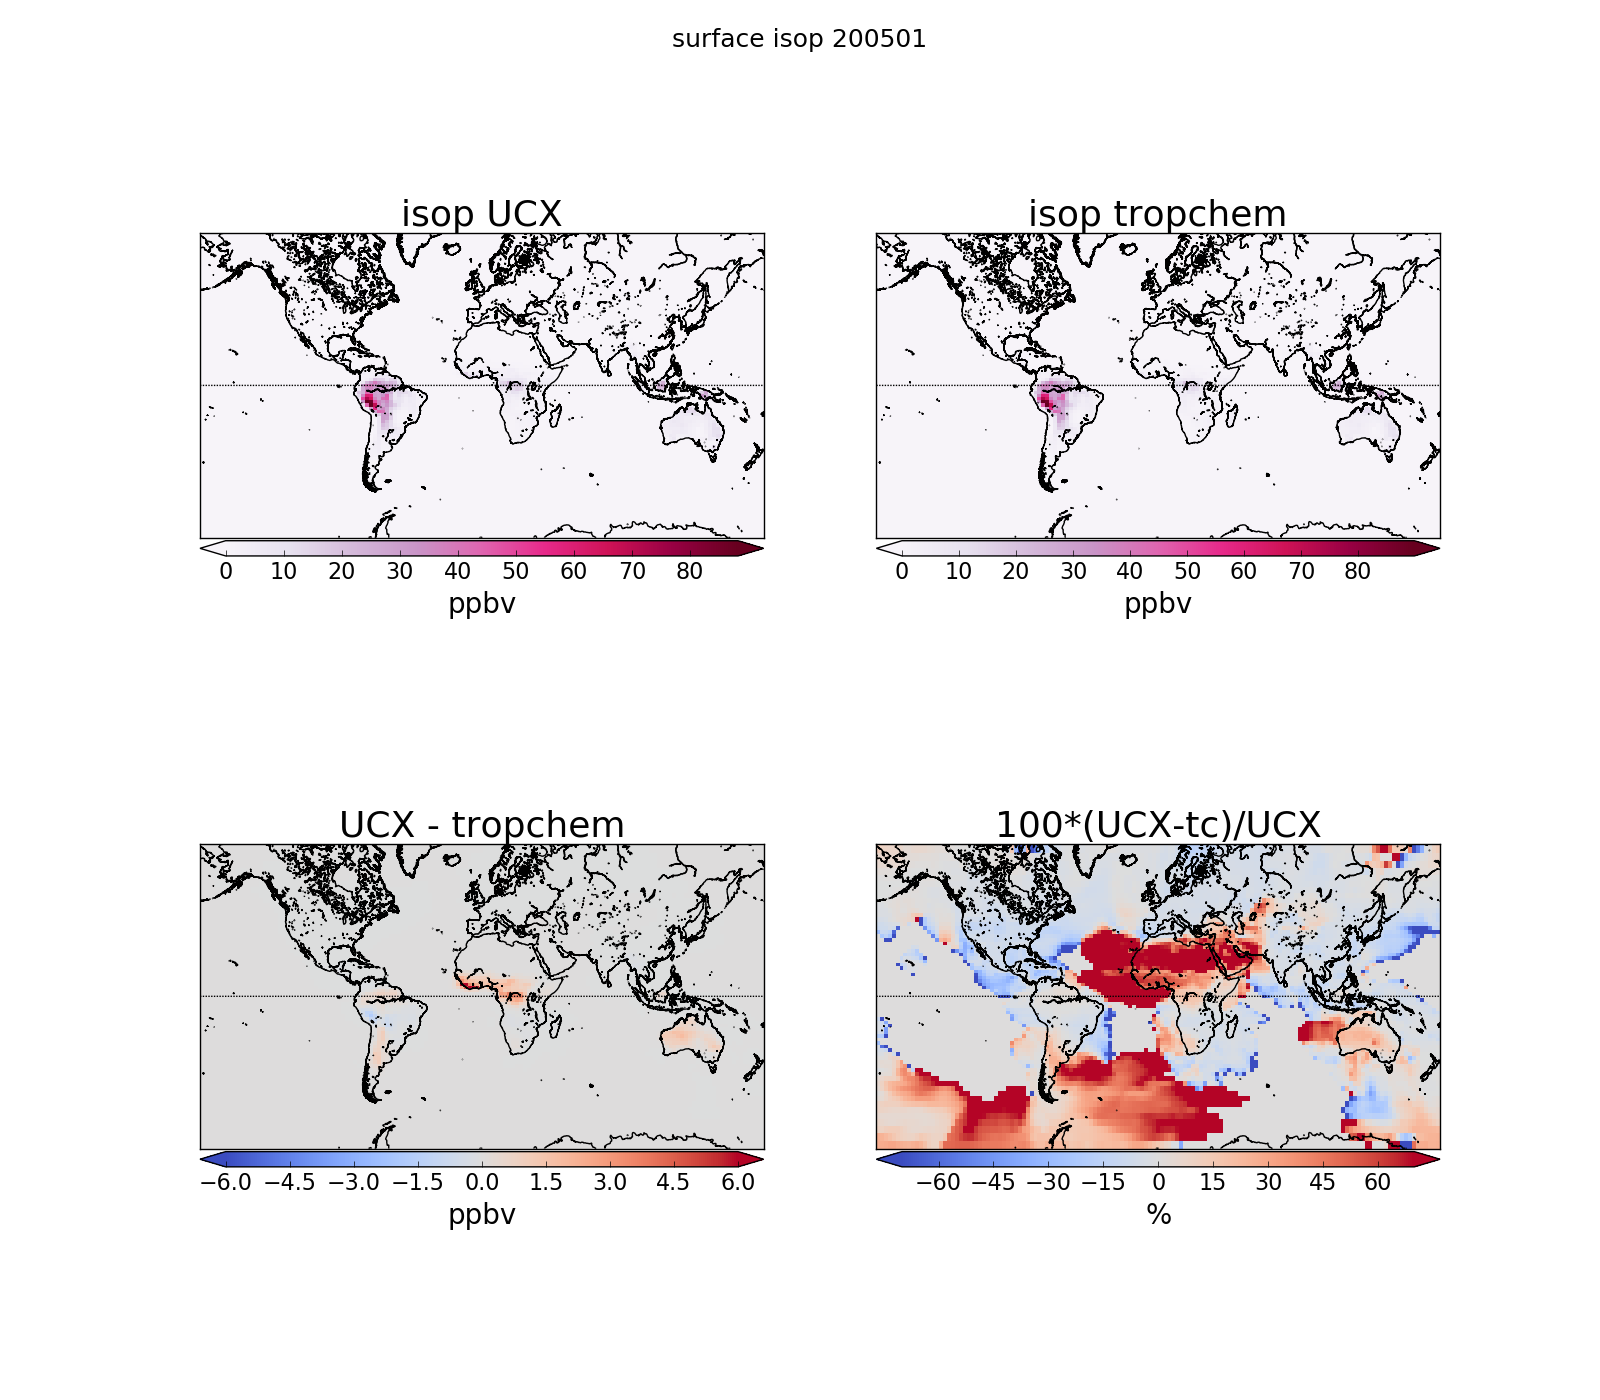
\includegraphics[width=\textwidth]{Figures/OMI_link/GC/UCX_vs_trp_glob_200501_isop_rerun.png}
        \caption{ %
          As figure \ref{Model:GC:running:fig_UCXvsTrop_HCHO}, except looking at isoprene. 
        }      
        \label{Model:GC:running:fig_UCXvsTrop_Isop}
      \end{figure}
      
      
      Figure TODO: shows the columns for isoprene and HCHO simulated by our two mechanisms over Australia in January of 2005.
      The differences are minimal compared to other uncertainties in both AMF calculation and emissions estimation.
      
      
      TODO: The difference in isoprene between UCX and tropchem is likely caused by differences in the modelled radiation reaching the troposphere due to differences in simulated ozone in the stratosphere.
      With higher stratospheric ozone levels, less radiation would reach the troposphere, changing the photochemistry.
      Figure \ref{Model:GC:running:fig_UCXvsTrop_O3} shows the total column ozone between UCX and non-UCX runs, we can see that UCX has TODO: less or more ozone over Australia/USA in January.
      
      \begin{figure}%[!htbp]
        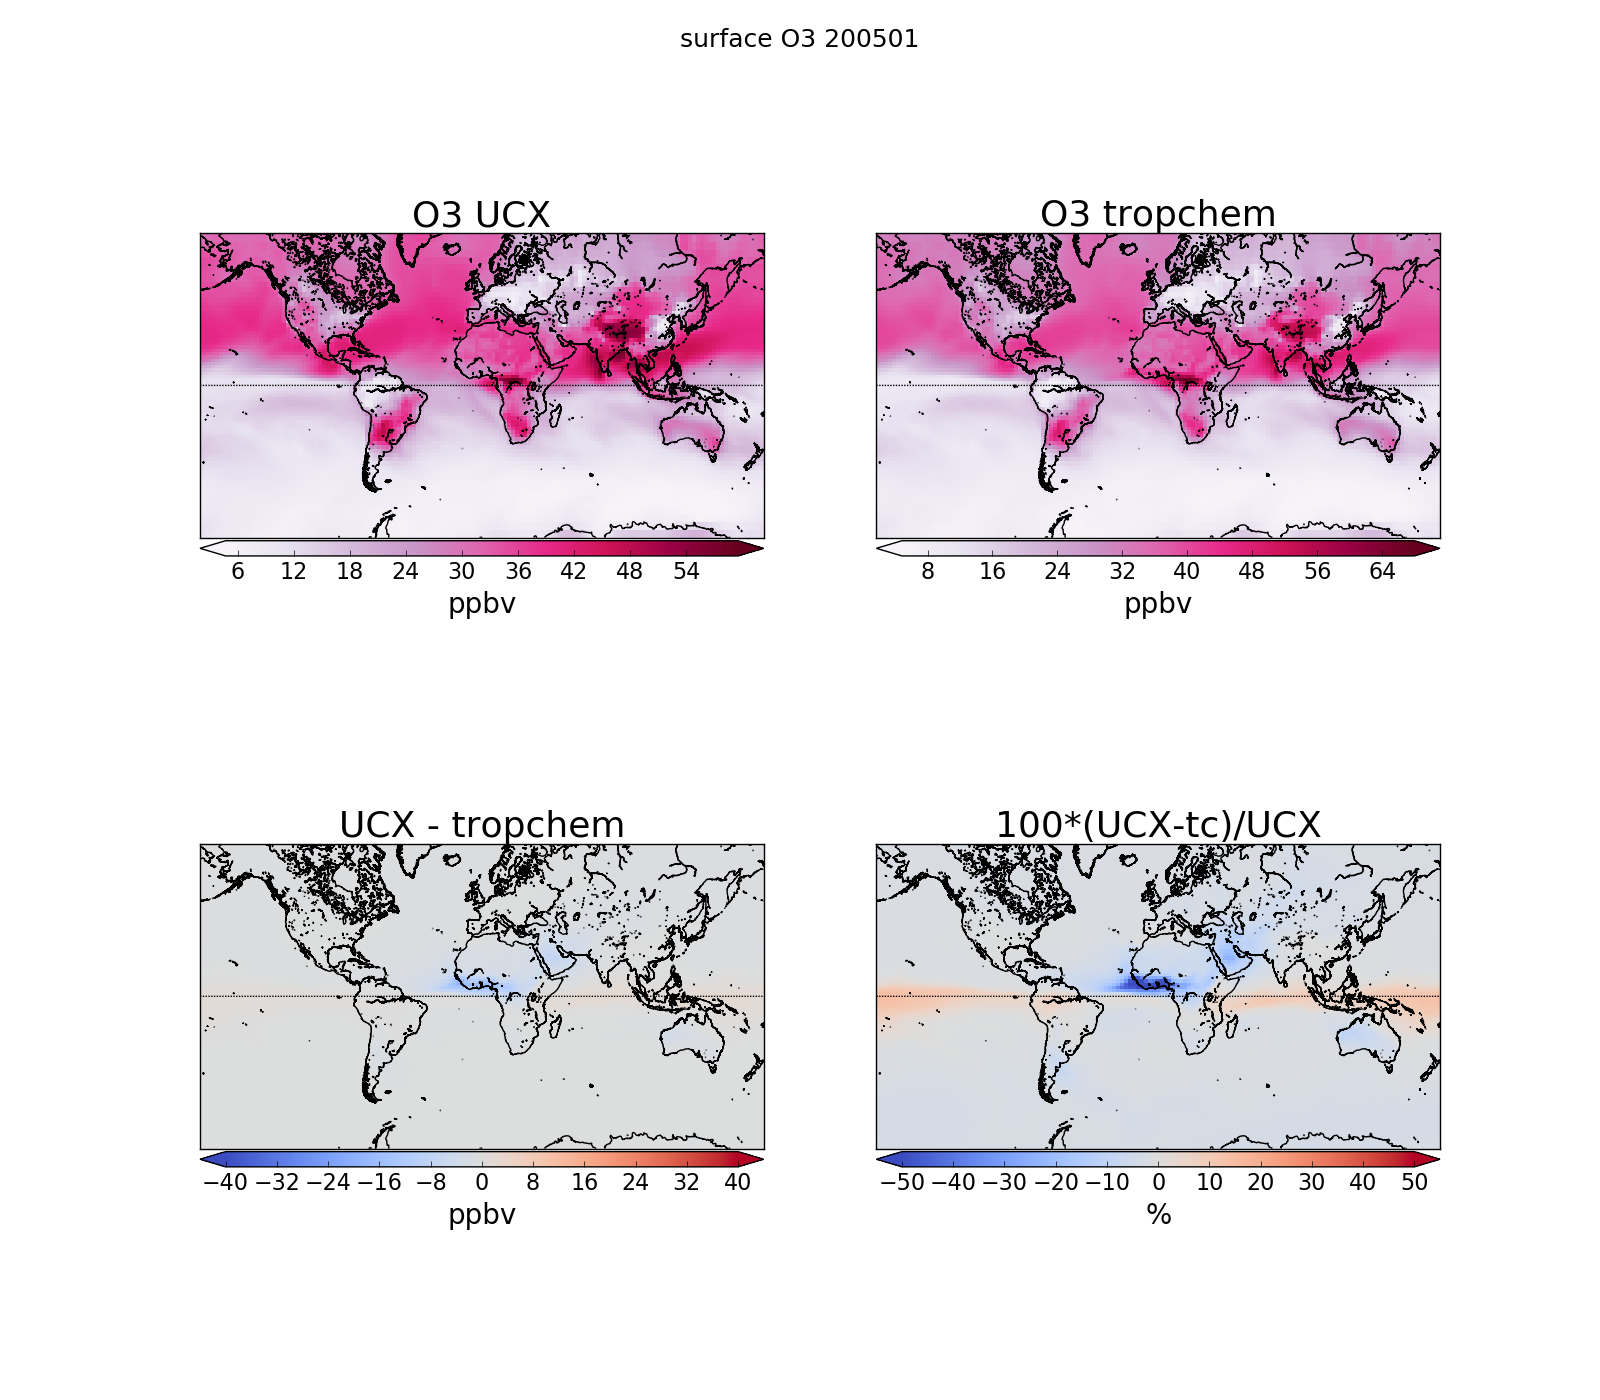
\includegraphics[width=\textwidth]{Figures/OMI_link/GC/UCX_vs_trp_glob_200501_O3_rerun.png}
        \caption{%
          As figure \ref{Model:GC:running:fig_UCXvsTrop_HCHO}, except looking at ozone. 
        }
        \label{Model:GC:running:fig_UCXvsTrop_O3}
      \end{figure}
  
  \subsection{GEOS-Chem outputs}
    \label{Model:GC:outputs}
    There are various outputs available when running GEOS-Chem, which require understanding in order to compare with observations.
    % Default time step and resolution of GC outputs
    GEOS-Chem in this thesis is run with a 15 minute time step for both chemistry and transport, at 2x2.5\degr horizontal resolution over 47 vertical levels.
    Generally output is the average of these time steps either over an entire month, or else per day.
    
    In my work when estimating model yields of isoprene to HCHO, I use daily averaged HCHO columns and compare them to colocated isoprene emissions from MEGAN.
    Optionally one can save high temporally resolved data for a single (or list of) column(s).
    I've used this diagnostic to compare modelled ozone with ozonesonde profiles at three sonde release sites discussed in Chapter \ref{Ozone}.
    
    
    \begin{description}
      \item[Satellite overpass]%
        is output from averaging over a window of local time for each gridbox. 
        This output allows comparison with satellite measurements, which overpass at the same local time every day.
        This diagnostic allows easier analysis of model data against a satellite as one can match the output with the satellite's overpass time.
        Output averaged between 1300-1400 LT is saved to allow comparisons with Aura satellite measurements, as Aura overpasses at $\sim$1330 LT each day.
        This has been performed by others \parencite[eg.][]{Jin2017}.
      \item[HEMCO diagnostics]%
        % Local time offsets
        In order to get hourly MEGAN modelled isoprene emissions, HEMCO (the module of GEOS-Chem dealing with emissions inventories) diagnostic output was created.
        When working with globally gridded data, handling local time offsets becomes more important.
        The hourly output emissions of isoprene is saved using GMT, which needs to be offset based on longitude in order to retrieve local time.
        I do this by setting up a latitude by longitude array which matches the horizontal resolution of the data, filling each gridbox with it's local time offset.
        This offset is determined as one hour per 15 degrees (since 360 degrees is 24 hours), and then used to retrieve global data at any specific local time.
        The retrieval of a daily local time global array is done by index matching the GMT+LT (modulo 24) with the desired hour on this grid over the 24 GMT hours.
        are the emissions TODO: averaged or instantaneous? in each gridbox, which I've stored for each 3 hours.
      \item[Tracer averages]%
        are daily or monthly averaged gridbox concentrations.
      
    \end{description}
     
      
\section{Measurement Techniques}
  \label{Model:Meas}
  While I have not made any measurements myself, it is important to understand the techniques used in datasets I have utilised in order to understand possible anomalous datapoints or trends.
  % Measurement difficulties
  In-situ measurements contain errors, and depending on the device used and chemical being measured this error can be significant.
  The major sources of uncertainty in measurement techniques included interference from non-target compounds and under-reporting \parencite[eg.][]{Dunne2017}.
  Overall isoprene uncertainty in measurements analysed by \textcite{Dunne2017} was a factor of 1.5 to 2.
  This can feed into uncertainties in modelling and satellite retrievals, as verification and correlations are affected.
  
  \subsection{DOAS}
    \label{Model:Meas:DOAS}
  
    %TODO: is some of this is repeated in isoprene chapter satellite section.
    The DOAS technique uses solar radiation absorption spectra to measure trace gases through paths of light.
    Beer's law states that $ T = I/I_0 = e^{-\tau} $ with T being transmittance, $\tau$ being optical depth, and I, I$_0$ being radiant flux received at instrument and emitted at source respectively.
    From $ \tau_i = \int \rho_i \beta_i ds $ we get:
    $$ I = I_0 \exp {\left( \Sigma_i \int \rho_i \beta_i ds \right) } $$
    Where i represents a chemical species index, $\rho$ is a species density(molecules per cm$^3$), $\beta$ is the scattering and absorption cross section area (cm$^2$), and the integral over ds represents integration over the path from light source to instrument.
    $\tau$ can be described using the attenuation cross section (the attenuation coefficient divided by its number density), with the following relation:
    \begin{equation*}
      \tau = \int_0^l \alpha(z)\eta(z)\mathrm{d}z
    \end{equation*}
    where $\alpha(z)$ and $\eta(z)$ represent absorption cross section in m$^2$ molecule$^{-1}$, and number density in molecules m$^{-3}$ respectively, and \textit{l} represents the length of the medium (in this case the path through which the light travels). 
    
    % Optical depth through the atmosphere
    Another way of describing optical depth, also called optical thickness, is the natural logarithm of the ratio of incident radiant power to transmitted radiant power through a material.
    In the atmosphere we are interested in the optical depth of various chemical species, and we use incoming solar radiation to determine this.
    The difference between solar radiation at the top of the atmosphere and the Earth's surface defines the atmospheric optical depth along the path of observation.
    \begin{equation*}
      \tau = \ln{\frac{\phi_e^i}{\phi_e^t}}
    \end{equation*}
    where $\phi_e^i$ is radiant flux seen at the earth surface, $\phi_e^t$ is the solar radiant flux which arrives at the top of the atmosphere.
    In the atmosphere, optical depth can be due to several factors including scattering, chemical absorbance, and aerosols.
    
  \subsection{Satellites}
  \label{Model:Meas:sat}
    
    % Satellites use DOAS for trace gases which we are interested in, which includes 
    In order to detect trace gases such as HCHO, satellites use a DOAS based technique to detect concentrations along the path of light which reaches the satellite instrument.
    This requires chemical transport and radiative transfer models used to transform the non-vertical light path into vertical column amounts.
    Measurements done using DOAS often apply a forward radiative transfer model (RTM) such as LIDORT (see section \ref{Model:Meas:sat:LIDORT}) in order to determine a trace gas's radiative properties at various altitudes.
    The forward RTM used for satellite data products also involves functions representing extinction from Mie and Rayleigh scattering, and the efficiency of these on intensities from the trace gas under inspection, as well as accounting for (often estimated) atmospheric parameters such as albedo.
    
    
    Rayleigh and Mie scattering describe two kinds of particle effects on radiation passing through a medium.
    Rayleigh scattering is heavily wavelength dependent, and is the dominant form of scattering from particles up to roughly one tenth of the wavelength of the light.
    Mie scattering is more dominant from larger particles, and has less wavelength dependence.
    %These scattering functions are described in detail at (maybe TODO:section? reference?).
    The effects of scattering are what gives us the information about substances in the atmosphere.
    The different particles and gases in the air have various properties which affect remote sensing devices such as a satellite, making them more or less sensitive at certain altitudes for detecting various species \parencite[e.g.]{Martin2002}.
    
    Satellites record near nadir (vertical) reflected spectra between around 250-700~nm split into spectral components at around $0.3$~nm in order to calculate trace gases including O$_3$, NO$_2$, and HCHO (eg: \textcite{Leue2001}).
    Several public data servers are available which include products from satellites, including NASAs Earthdata portal (\url{https://earthdata.nasa.gov/}) and the Belgian Institute for Space Aeronomy (IASB-BIRA) Aeronomie site (\url{http://h2co.aeronomie.be/}).
    
    Satellite measurements are generally performed using spectral fitting followed by conversion to vertical column densities.
    %The use of multiple satellites can even be used to detect intradiel concentrations in trace gas columns, as shown in \textcite{Stavrakou2015} using OMI and GOME-2 measurements, which have respective overpass times of 1330 and 0930 LT.
    Instruments including MODIS on board the AQUA and TERRA satellites are also able to determine aerosol optical depth (AOD), a measure of atmospheric scatter and absorbance. 
    An AOD of under 0.05 indicates a clear sky, while values of 1 or greater indicate increasingly hazy conditions.
    This is important in order to determine where measurements from other instruments may be compromised by high interference.
    Satellite measured AOD requires validation by more accurate ground based instruments like those of AERONET which uses more than 200 sun photometers scattered globally.
    
    Soon even more HCHO data will be available in the form of geostationary satellite measurements (\textcite{Kwon2017}).
    \textcite{Kwon2017} examine simulated geostationary measurements against GEOS-Chem column simulations to determine the most important instrument sensitivities.
    Geostationary satellites can provide temporally rich measurements over an area, as they are not sweeping around the earth but fixed relative to one latitude and longitude.
    
    \subsubsection{LIDORT}
      \ref{Model:Meas:sat:LIDORT}
      
      %http://www.rtslidort.com/about_publications.html
      LIDORT is a model of LInearized Discrete Ordinate Radiative Transfer, used to determine backscatter intensities and weighting functions at arbitrary elevation angles \parencite{Spurr2001}.
      The model solves radiative transfer equations and can be used to determine various atmospheric column measurement attributes such as optical depth, ring effects, and scattering.
      These radiative properties (or at least estimates thereof) are required when measuring trace gases in the atmosphere through a long path such as seen by satellites \parencite[eg.][]{Palmer2001,Martin2002a,DeSmedt2015,Abad2015}.
    
      
    
    \subsubsection{OMI}
    
      The OMI instrument on board AURA has been active since July 2005, it records spectra from 264-504~nm using an array of 60 detectors with mid-resolution (0.4-0.6~nm).
      This band of wavelengths allows measurments of trace gases including O$_3$, NO$_2$, SO$_2$, HCHO, and various other quantities like surface UV radiation.
      Recently \textcite{Schenkeveld2017} analysed the performance over time of the instrument and found irradiance degradation of 3-8\%, changed radiances of 1-2\%, and a stable wavelength calibration within 0.005-0.020~nm.
      They also provide a very nice summary of the OMI instrument copied here in Fig. \ref{LR:HCHO:Sat:fig_Shenkeveld_OMI_summary}, as it shows the instruments spectral, temporal, and spatial resolutions.
      These changes are measured excluding the row anomaly (RA) effect, which is relatively stable since 2011, although it is still growing and remains the most serious concern.
      An analysis of the row anomaly by \textcite{Huang2017} state that OMI ozone columns remain suitable for scientific use, with recommendation for further evaluation.
      And analysis of OMI output by \textcite{Schenkeveld2017} concludes that data is still of high quality and will deliver useful information for 5-10 more years, with radiances only changing by $1-2\%$ outside of RA impacted areas.
      The RA began in June 2007, with some cross-track rows seemingly blocked. The most likely cause is some instrument insulation partially obscuring the radiance port (\textcite{Schenkeveld2017}).
      
      \begin{figure}
        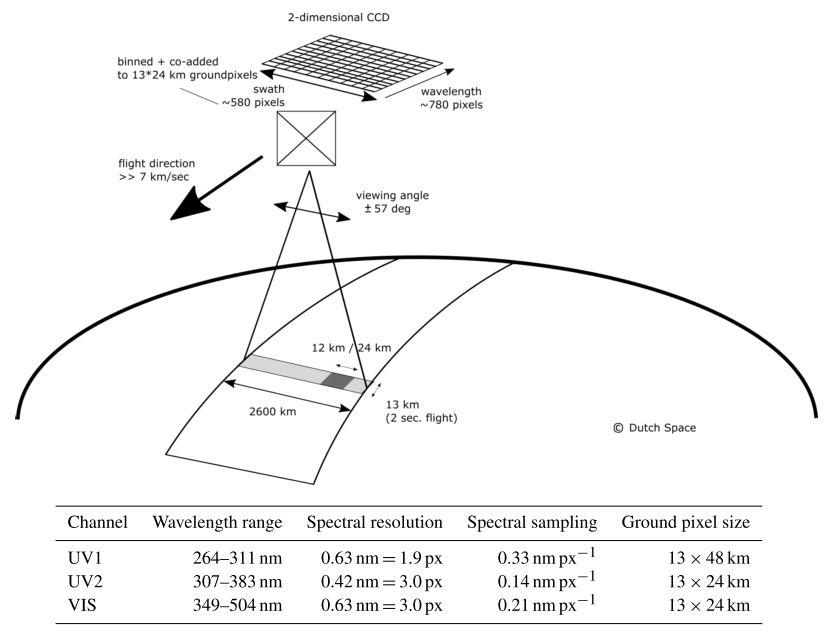
\includegraphics[width=\textwidth]{Figures/Shenkeveld_OMI_summary.png}
        \caption{ %
          Figure 1 and Table 1 from \textcite{Schenkeveld2017}, with the following caption ``An impression of OMI flying over the Earth.
          The spectrum of a ground pixel is projected on the wavelength dimension of the charge-coupled device (CCD; the columns). 
          The cross-track ground pixels are projected on the swath dimension of the CCD (the rows).
          The forward speed of 7~kms$^{-1}$ and an exposure time of 2~s lead to a ground pixel size of 13~km in the flight direction.
          The viewing angle of 114\degr leads to a swath width on the ground of 2600~km.''
          The table shows the optical properties for OMIs three channels.}
      \label{LR:HCHO:Sat:fig_Shenkeveld_OMI_summary}
      \end{figure}
        
    \subsubsection{Air mass factor (AMF)}
      
      % what satellite amfs are, and what they do
      An AMF characterises measurement sensitivity to a trace gas at various altitudes \cite[e.g.]{Palmer2001}.
      \textcite{Lorente2017} show that AMF calculations can be the largest source of unertainty in satellite measurements.
      Another way of describing AMFs are as measures of how radiance at the top of the atmosphere (TOA) changes with trace gas optical depths at specific altitudes (\textcite{Lorente2017}).
      Calculation of the AMF is important as it is multiplied against the estimated slant columns in order to give vertical column amounts.
      To convert the trace gas profile from a reflected solar radiance column (slanted along the light path) into a purely vertical column requires calculations of an air mass factor (AMF).
      In satellite data, the AMF is typically a scalar value for each horizontal grid point which will equal the ratio of the total vertical column density to the total slant column density.
      This value requires calculations to account for instrument sensitivities to various wavelengths over resolved altitudes, and is unique for each trace gas under consideration.
      
      %how do we get an AMF?
      DOAS retrieval columns are an integration of a trace gas over the instruments viewing path, in order to convert this total to a vertically distributed column a few assumptions and estimates are required. 
      The vertical profile of a trace gas is assumed or estimated via a CTM, while its' scattering and radiative properties are calculated at all altitudes using an RTM. 
      These properties are combined into a single array called the AMF.
      Two examples of this are GOME-2 products on the MetOp-A satellite (\url{http://atmos.caf.dlr.de/gome/product_hcho.html}) and OMI products which use IMAGESv2 combined with LIDORT and GEOS-Chem with LIDORT for product processing respectively \parencite{Chance2002, Abad2015}.
      AMFs are unique to each trace gas and due to their complexity and the influence of cloud cover they remain one of the larger error sources in remote sensing of BVOCs \parencite{Palmer2001,Millet2006}).
      
      % averaging kernal relation to amf, why amfs are important when comparing data
      Related to the AMF is the averaging kernal (AK), which is used to handle instrument measurements which are sensitive to concentrations at different altitudes in the atmosphere.
      DOAS methods can be heavily influenced by the initial estimates of a trace gas profile (the a priori) which is often produced by modelling, so when comparing models of these trace gases to satellite measurements extra care needs to be taken to avoid introducing bias from differing a priori assumptions.
      One way to remove these a priori influences is through the satellites AK (or by using AMFs), which takes into account the vertical profile of the modelled trace gas and instrument sensitivity to the trace gas (\textcite{Eskes2003, Palmer2001}).
      % TODO read and note this paper:
      \textcite{Lamsal2014} recommends that when comparing satellite data to models, the AMF should first be recalculated using the model as an a priori.
      This is in order to remove any a priori bias between model and satellite columns.
      Another way of removing this bias is through deconvolution ($\Omega = AK \times VC_{satellite} + \times (I - AK) VC_{a priori}$) of the averaging kernal (AK) of the satellite instrument.
      The AK represents sensitivities to each species at multiple altitudes through the atmosphere and in the case of OMI, can be approximated from the scattering weights ($\omega(z)$) function as follows:
      \begin{equation} \label{ch_HCHO:eqn:AKfromw}
      AK(z) = \frac{\omega(z)}{AMF}
      \end{equation}
      Note that this is an approximation for the OMI product, which does not include the AK but does include the $\omega$ and AMF, as explained in \textcite{Abad2015}.
      
      % How omi gets its AMF
      The latest OMI algorithm uses a shape factor determined from GEOS-Chem using 47 vertical levels at monthly temporal resolution and 2$^{\circ}$ latitude by 2.5$^{\circ}$ longitude horizontal resolution \parencite{Abad2015}.
      The GEOS-Chem model has been substantially updated since then, and using the more recent version $V10.01$ to recalculate the AMF is performed within this thesis, details are shown in section \ref{Model:omiRecalc}.
      
    \subsubsection{Uncertainties}
      %Satellite Errors
      While satellite data is effective at covering huge areas (the entire earth) it only exists at a particular time of day, is subject to cloud cover, and generally does not have fine horizontal or vertical resolution.
      Concentrations retrieved by satellites have large uncertainties, which arise in the process of transforming spectra to total column measurements, as well as instrument degradation (satellite instruments are hard to tinker with once they are launched).
      Uncertainty in transforming satellite spectra comes from a range of things, including measurement difficulties introduced by clouds, and instrument sensitivity to particular aerosols \parencite{Millet2006}.
      Many products require analysis of cloud and aerosol properties in order to estimate concentration or total column amounts \parencite{Palmer2001,Palmer2003, Marais2012, Vasilkov2017}.
      The main source of error in satellite retrievals of HCHO are due to instrument detection sensitivities, and the vertical multiplication factor \parencite{Millet2006}.
      % amf agreements between groups, but sensitive to a priori
      Calculations of the AMF performed by different groups tend to agree fairly well, as long as all the a priori and ancilliary data is similar.
      Large differences can occur depending on the a priori vertical profile, trace gas concentrations, and cloud properties \parencite{Lorent2017}.
      Choice of RTM and interpolation operations have a relatively small affect compared to the assumed state of the atmosphere, with high structural uncertainty introduced at this stage of AMF calculation - as shown in \textcite{Lorent2017}.
      
      There are two types of measurement error, arguably the worst of these is systematic error (or bias) which normally indicates a problem in calculation or instrumentation.
      If the systematic error is known, it can be corrected for by either offsetting data in the opposite direction, or else fixing the cause.
      A proper fix can only be performed if the sources of error are known and there is a way of correcting or bypassing it.
      Random error is the other type (often reported as some function of a datasets variance, or uncertainty), and this can be reduced through averaging either spatially or temporally. 
      By taking the average of several measurements, any random error can be reduced by a factor of one over the square root of the number of measurements.
      This is done frequently for satellite measurements of trace gases (which are often near to the detection limit over much of the globe).
      For example: \textcite{Vigouroux2009} reduce the measurement uncertainty (in SCIAMACHY HCHO columns) by at least a factor of 4 through averaging daily over roughly 500km around Saint-Denis, and only using days with at least 20 good measurements.
      
      %% grid size and averaging
      Satellite measurements of HCHO are relatively uncertain, however this can be improved by averaging over larger grid boxes or longer time scales.
      An example of this can be seen in \textcite{Dufour2009}, where monthly averaging is used to decrease the measurements uncertainty.
      %They examine HCHO in Europe, which is low; near the detection limit of satellite measurements.
      %Taking monthly averages allows enough certainty that useful inversions can be determined to estimate the source emissions of HCHO.
      The finer nadir resolution of OMI (13 by 24~km${^2}$) compared to other satellites reduces cloud influence \parencite{Millet2006, Millet2008}.
      Although the uncertainty in each pixel is $\sim 2 \times 10^{16}$, which is $5 \times$ higher than GOME, there are $\sim 100-200 \times $ as many measurements due to the smaller footprint and better temporal resolution of OMI, which allows a greater reduction of uncertainty with averaging \parencite{Chance2002,Millet2008}.
      % Uncertainty in OMI pixels measurements
      Uncertainty in a single pixel for OMI is roughly the same magnitude as HCHO background levels.
      The top row in figure \ref{Model:Meas:sat:fig_OMI_uncertainty} shows OMI HCHO columns binned to at 0.25\degr longitude by 0.3125\degr latitude averaged over one day, one month, and one month after filtering.
      Row two shows uncertainty of the satellite data after averaging.
      It's clear that one day of satellite data is too uncertain when binned at 0.25x0.3125\degr horizontal resolution, however after a month with or without filtering the uncertainties become manageable.
      % TODO: Several methods of uncertainty where?
      %There are several methods of calculating this, one of which is used here and compared against the provided uncertainty (TODO) as shown in Section \ref{}.
      If we assume the uncertainty is random error, and not bias introduced through calculation techniques, then we are able to reduce the uncertainty through averaging.
      Random error can be reduced by temporal and/or spatial averaging, decreasing uncertainty by a factor of $1/\sqrt{N}$ where N is the number of observations being averaged.
      High resolution low detection limit estimates can be built up using ``oversampling'', which averages satellite measurements over time \parencite[eg.][]{Zhu2014}.
      %A good example can be seen in \textcite{Zhu2014} where 0.2$^{\circ}$ by 0.2$^{\circ}$ resolution with high enough sensitivity to see anthropogenic HCHO is acheived with three summers worth of satellite data.
      
      % Figure from tests.py
      \mypic{Figures/OMI_link/Uncertainty_OMI_200501.png}{}{\label{Model:Meas:sat:fig_OMI_uncertainty}}
      
%      \begin{figure}
%        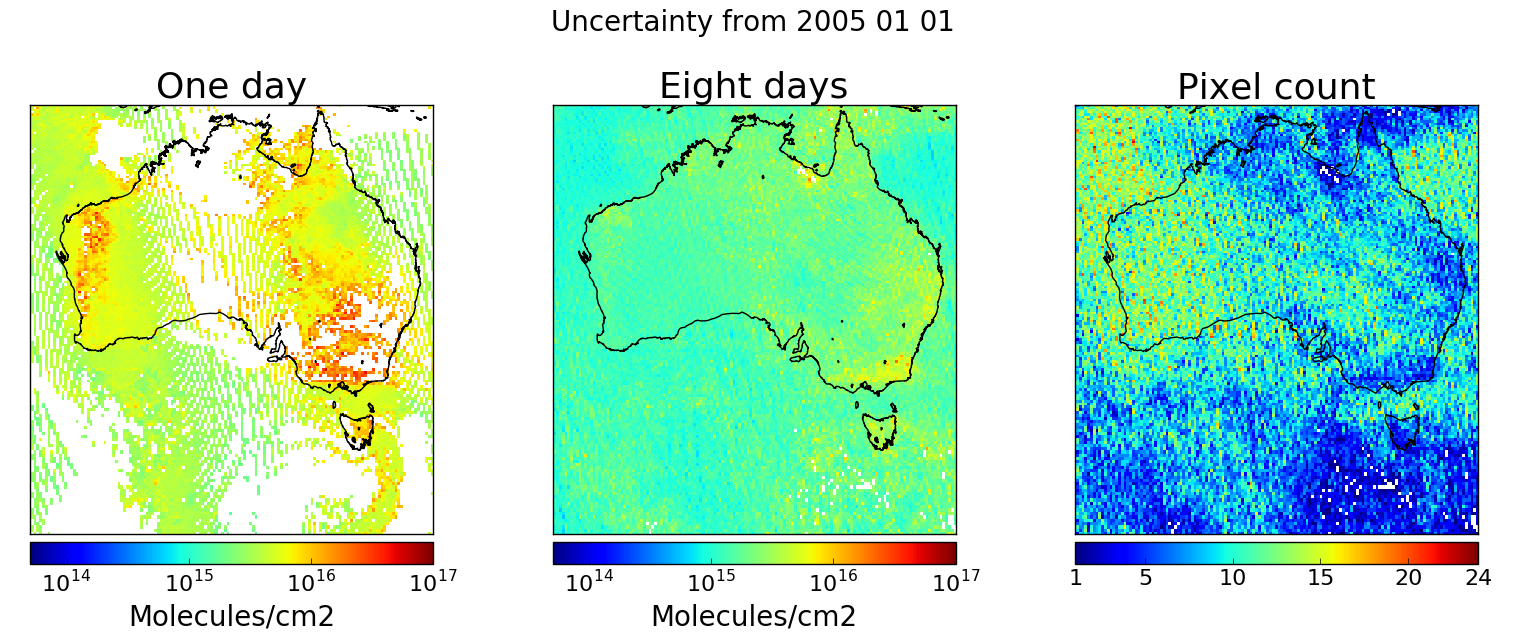
\includegraphics[width=\textwidth]{Figures/HCHO/Uncertainty.png}
%        \caption{%
%          OMI uncertainty before and after gridding and averaging 8 days from Jan 1 2005 to Jan 8 2005.
%          The third panel shows the number of pixels in each grid box after 8 days of averaging, before accounting for fire.
%        }
%        \label{Model:Meas:sat:fig_averagingUncertainty}
%      \end{figure}
      
      %% SURFACE CONDITIONS AND CLOUDS
      In cloudy, hazy or polluted areas measurements are more difficult to analyse (\cite[e.g.][]{Palmer2003,Marais2014}).
      Recent work by \textcite{Vasilkov2017} showed that updating how the surface reflectivity is incorporated into satellite measurements can change the retrievals by 50~\% in polluted areas.
      With the satellite HCHO columns, we filter cloud fractions over 40\%, which introduces a clear-sky bias.
      This bias has been measured as a 13\% positive monthly mean bias by \textcite{Palmer2001, Surl2018}.
      
      %% BACKGROUND MEASUREMENTS
      In satellite HCHO products, concentrations over the remote pacific ocean are sometimes used to analyse faulty instrument readings.
      This is due to the expected invariance of HCHO over this region.
      For instance GOME (an instrument which measures trace gases on board the ERS-2) corrects for an instrument artifact using modelled HCHO over the remote pacific \parencite{Shim2005}.
      OMI HCHO products use a similar technique to account for sensor plate drift and changing bromine sensitivity \parencite{Abad2015}.
      Uncertainty in the OMI satellite instrument is calculated by the Smithsonian Astrophysical Observatory (SAO) group using the uncertainty in backscattered radiation retrievals \parencite{Abad2015, Abad2016}.
      Another method of calculating the uncertainty is used by the Belgian Institute for Space Aeronomy (BIRA) group, who determine uncertainty from the standard deviation of HCHO over the remote pacific ocean \parencite{DeSmedt2012, DeSmedt2015}.
      
      
      %% EXAMPLES OF BIAS
      For many places the tropospheric column HCHO measured by satellite is biased low, \textcite{Zhu2016} examine six available datasets and show a bias of 20 - 51\% over south east USA when compared against a campaign of aircraft observations (SEAC$^4$RS).
      \textcite{DeSmedt2015} also found OMI and GOME2 observations were 20 - 40\% lower than ground based vertical profiles, and \textcite{Barkley2013} determine OMI to be 37\% low compared with aircraft measurements over Guyana.
      These bias can be corrected by improving the assumed a priori HCHO profiles which are used to calculate the AMFs of the satellite columns.
      \textcite{Millet2006} examine OMI HCHO columns over North America and determine overall uncertainty to be 40\%, with most of this coming from cloud interference.
      \textcite{Millet2008} shows that there also exists some latitude based bias, as well as a systematic offset between the OMI and GOME instruments.
      This does not appear to be due to the different overpass times of the two instruments.
      
      %% UNCERTAINTY CALCULATIONS
      
      A full analysis of the AMF uncertainty in OMI measurements, as well as the structural uncertainty (between different systems of calculations applied to the same data) is performed by \textcite{Lorente2017}.
      They determine the structural uncertainty on seven AMF calculation approaches used by different retrieval groups.
      They show that in scenarios where the gas is enhanced in the lower troposphere, AMF calculation is the largest uncertainty in satellite measurements.
      In polluted environments the structural uncertainty is estimated at 42~\%, or 31~\% over unpolluted environments.
      The importance of a priori and ancillary data (such as surface albedo and cloud top height) is also shown, as it sharply affects the structural uncertainty.
      
      

\section{Recalculation of OMI HCHO}
  \label{Model:omiRecalc}
  
  % what is AMF, Omega_V and Omega_S
  The AMF is needed to transform the slant column (SC) viewed by the satellite into a vertical column ($\Omega$):
  \begin{equation}
    \label{Model:omiRecalc:eqn_AMFratio}
    AMF = \frac{SC}{\Omega} %= \frac{\tau_s}{\tau_v}
  \end{equation}
  A slant or vertical column is expressed in molecules cm$^{-2}$.
  % Reiteration of why we recalculate AMFs
  OMI HCHO vertical columns are calculated using modelled a priori HCHO profiles (see section \ref{Model:Datasets:OMHCHO}).
  When comparing satellite measurements against models it is important to recognise the impact of this a priori on the total column values.
  This is due to how the sensitivity of OMI (to HCHO and other trace gases) varies vertically throughout the atmosphere.
  When comparing OMI vertical columns ($\Oo$) to GEOS-Chem ($\Og$), the satellite AMF needs to be recalculated using GEOS-Chem modelled vertical gas profiles as the a prioris.
  Without performing this step a bias between modelled and measured total column values may be due to the a priori rather than chemistry or measurements \parencite{Palmer2001, Lamsal2014}.
  
  % Very brief outline
  Here, two new AMFs are calculated, both using GEOS-Chem HCHO profiles as the new a priori. 
  The first AMF (AMF$_{GC}$) uses the original satellite scattering weights while recalculating the shape factor, whereas the second AMF (AMF$_{PP}$) also recalculates scattering weights.
  AMF$_{PP}$ is created using code initially written by Professor P. Palmer (see sections \ref{Model:omiRecalc:ShapeFactor} and \ref{Model:omiRecalc:ppcode} for more details).
  A reference sector correction is determined using the method described in \textcite{Abad2016}, (see section \ref{Model:omiRecalc:RSC}).
  This correction is unique for each of the 60 \textit{measurement tracks} used by OMI.
  Finally the correction is applied to each pixel to create the corrected vertical column. 
  The end product is three sets of corrected vertical columns (VCC): the original ($\Ooc$), one using GEOS-Chem shape factors ($\Ogc$), and one from Palmer's code ($\Opc$).
  
  \subsection{Outline}
    \label{Model:omiRecalc:outline}
    
    % Summary of actual actions taken:
    Here is an outline in computational order of what takes place when recalculating the $\Omega$ from OMI.
    \begin{enumerate}
      \item GEOS-Chem satellite overpass output (see section \ref{Model:GC:outputs}) is used to create new shape factors (S$_z$ and S$_\sigma$).
      \begin{enumerate}
        \item Pressure edges and geometric midpoints are determined, along with altitudes (\textit{z}), and box heights (H).
        \item Number density and mixing ratio of HCHO ($n_{HCHO}$, $C_{HCHO}$ respectively) are taken or created from model outputs HCHO(ppb) and air density (molec/cm3)
        \item Total column HCHO from GEOS-Chem ($\Og$) is calculated $\Og = \Sigma_z \left(n_{HCHO}(z) \times H(z) \right)$, along with total column air ($\Omega_{A}$, calculated similarly)
        \item The shape factor S$_z(z)$ is calculated on each altitude $S_z(z) = n_{HCHO} / \Omega_{HCHO}$.
        \item Pressures (\textit{p})are used to create sigma coordinates $\sigma(z) = (p(z) - p_{TOA}) / (p(0)-p_{TOA})$
        \item S$_\sigma(z)$ is calculated on each altitude: $S_\sigma(z) = C_{HCHO}(z) \times \Omega_A / \Omega_{HCHO}$
      \end{enumerate}
      \item Satellite pixels (SC, scattering weights ($\omega(z)$), pressure levels, latitude and longitude) are read from the OMHCHO dataset.
      \item For each pixel, a new AMF (AMF$_{GC}$)is created using the GEOS-Chem shape factors and satellite scattering weights.
      \begin{enumerate}
        \item scattering weights ($\omega$) are interpolated onto the same vertical dimensions (\textit{z} and $\sigma$) as the shape factors.
        \item Integration (approximated using rectangular method) is performed along the vertical dimension to calculate the new AMF on both coordinate systems.
        \begin{align}
          AMF_z &= \Sigma_z \left(\omega(z) \times S_z(z) \times H(z)\right) \\
          AMF_s &= \Sigma_{\sigma} \left(\omega(\sigma) \times S_{\sigma}(\sigma) \times d\sigma \right)
        \end{align}
      \end{enumerate}
      \item These two AMFs represent the same thing using different coordinates. Either one can be used as the AMF$_{GC}$.
      \item The AMF$_{PP}$ (created separately) and AMF$_{GC}$ are used to determine the new vertical columns ($\Op$, $\Og$ respectively): $\Omega = SC/AMF$.
      \item A reference sector correction (RSC) is defined each day using these AMFs along with modelled HCHO over the remote pacific.
      \begin{enumerate}
        \item GEOS-Chem satellite overpass output ($\Omega_{GEOS-Chem}$ from 140{\degr}W to 160{\degr}W) are averaged monthly and longitudinally to provide a modelled reference sector $\Omega_0[lat]$.
        \item The modelled reference slant columns (\textit{MRSC}) are calculated using $MRSC = \Omega_0 \times AMF$ for each AMF.
        \item For each satellite pixel between 140{\degr}W and 160{\degr}W, the correction is calculated as the measured \textit{SC} minus the \textit{MRSC} at the nearest latitude.
        \begin{equation*}
          corr[lat,track] = SC[lat,track] - MRSC[lat]
        \end{equation*}
        \item These corrections are binned by satellite detector (track: 1-60), and latitude (0.36\degr; 500 latitudes from 90{\degr}S to 90{\degr}N).
        \item The median entry of each bin is determined and this forms the RSC[lat,track]
      \end{enumerate}
      \item VCC are determined using $VCC = (SC - RSC[lat,track] )/AMF$ for each measured SC and using each AMF, with the RSC linearly interpolated to the latitude of the satellite pixel.
      \item The VCC (along with most of the pixel and GEOS-Chem data) are binned onto a 0.25\degr by 0.3125\degr grid along with how many pixels have been binned, and the average pixel uncertainty in product OMHCHORP.
    \end{enumerate}
  
    Figure \ref{Model:omiRecalc:fig_flow_omhchorp} shows an overview of how these profiles are used in this thesis.
    Output from GEOS-Chem is combined with OMHCHO swath data to produce a gridded HCHO file which contains HCHO vertical columns recalculated with GEOS-Chem a prioris.
    The output keeps the original AMF as well as those recalculated using GEOS-Chem (AMF$_{OMI}$, AMF$_{GC}$, and AMF$_{PP}$).
    Additionally, MOD14A1, OMAERUVd and OMNO2d data are used to create masks which are also stored in the OMHCHORP dataset.
    The creation of fire, smoke, and anthropogenic influence masks is described in section \ref{Model:Filter}.
    
    \mypic{Figures/Flow_Making_omhchorp.png}{Flow diagram showing how OMHCHO level two swath data is read, processed, and gridded in this thesis}{\label{Model:Datasets:OMHCHO:fig_flow_omhchorp}}
    
  \subsection{Reading satellite data}
    
    % Downloading the data
    First satellite slant columns of formaldehyde for the years January 1st, 2005 - April 1st, 2013 are downloaded (see section \ref{Model:Datasets:OMHCHO}).
    The data set used is from the Ozone Monitoring Instrument (OMI) on board the Aura satellite, as it has data for the entire time line and sufficiently covers the southern hemisphere.
    % Filters applied when reading
    When reading OMHCHO level 2 swath files, several factors are taken into account in order to filter uncertain and erroneous pixels.
    The process is outlined in figure  \ref{Model:Datasets:OMHCHO:fig_flow_omhchorp} for a single day.
    First all \textit{good} pixels (those with QA flag equal to 0) are read into a long list (roughly 1 million per day).
    These are then filtered by solar zenith angle (SZA) and latitude, similarly to other works \parencite[eg.]{Marais2012, Barkley2013, Bauwens2016, Zhu2016}.
    This filtering removes highly uncertain pixels, along with those for which instrument problems such as the OMI row anomaly (see section \ref{Model:Datasets:OMHCHO}) may have affected.
    
    % Actual filtering done
    Satellite measurements polewards of 60\degr north or south are removed as well as measurements with SZA greater than 60\degr.
    Pixels with a cloud fraction greater than 40\% are filtered out after RSC is created.
    Further filtering is performed to remove the measurements which are most likely to be unrealistic: those with column density outside the range $-0.5 \times 10^{16}$ to $10^{17} $\moleccm, as is performed by\textcite{Zhu2016}.
    This final filter is required due to currently unexplained large negative values which occur in the OMI HCHO product increasingly over time.
    Figure \ref{Model:omiRecalc:fig_OMI_negative_hist} shows how unfiltered HCHO columns are affected by a small set of highly negative values which heavily affect the mean column amount over any region.
    The histograms here show the negative (left) and positive (right) total column HCHO measurements from a subset of swaths over Australia, on the 18th of March 2013.
    The highly negative values can be seen around the $-10^{19}$~molecules cm$^{-2}$ region.
    
    \mypicw{0.7\textwidth}{Figures/AusOMHCHO_Hist_20130318.png}
    {Column density histograms for a subset of OMI swaths over Australia on the 18th of March 2013.
      Negative entries are shown in the left panel, positive in the right, note the different scale between negative and positive panels.}
    {\label{Model:omiRecalc:fig_OMI_negative_hist}}
    
    % Built in QA
    
    
    % reading pixels into a long list
    Each pixel and it's relevant data are saved in a long list, around $1.1$ million pixels per day.
    Additional information is added to each pixel, such as the new AMF calculated through replacing the a priori vertical profile with the newer GEOS-Chem simulated profile.
    The shape factors and scattering weights for each pixel lie along a z-axis which is vertically resolved to 47 layers.
    
    
    Finally the pixels which may be too cloudy are dealt with after the pixel has been used in determining the reference sector correction (see section \ref{Model:omiRecalc:RSC}), as is done in \textcite{Abad2015, DeSmedt2015}.
    Any pixel with a cloud fraction of greater than 40\% is removed, 
  
  % How we get the a priori 
  \subsection{Scattering weight and the shape factor}
    \label{Model:omiRecalc:ShapeFactor}
    
    %    % Method outline
    %    In order to visualise and analyse OMI HCHO columns slant columns are transformed into vertical columns. 
    %    This is done using AMF calculations, determined from the scattering weights and a priori estimates of HCHO vertical profiles.
    %    Radiative transfer modelling is required to determine instrument sensitivities throughout the atmosphere.
    %    Several of these required data are available from the satellite data products, including the scattering weights and the zenith angles required to determine an AMF at any particular measured point.
    In this section I describe how the shape factor can be used to recalculate OMI AMFs.
    The associated OMI per-pixel scattering weights are not changed in this calculation (unlike in section \ref{Model:omiRecalc:ppcode}).
    The satellite shape factor is replaced by GEOS-Chem's overpass time simulated HCHO profile, normalised and saved daily along with air density.
    
    % per pixel amf calculation
    OMI's a priori shape factor is based on the GEOS-Chem (v9) model, which uses 47 layers between the earth's surface and the top of the atmosphere using a pressure-eta hybrid (the actual values are shown in table \ref{app_a:tab:gc_47_vgrid}).
    The equations and method of recalculating this a priori shape factor with the newer GEOS-Chem V10.01 code is layed out in this section.
    For each pixel the shape factor used in the AMF is recalculated using GEOS-Chem by following the method layed out initially in \textcite{Palmer2001}.
    
    % Beer lambert
    The Beer-Lambert law of extinction allows spectroscopic measurement of absorbing chemical species (absorbers) in the atmosphere:
    \begin{equation} \label{ch_HCHO:eqn:beerlambert}
    I_B = I_{B_0} e^{-\tau_s}
    \end{equation}
    where I$_B$, I$_{B_0}$ is backscattered intensity with and without the absorber respectively, and $\tau_s$ is the optical thickness of the slant column absorber (see section \ref{Model:Meas:DOAS}).
    
    The AMF is needed to transform the slant column, as viewed by the satellite, into a vertical column:
    \begin{equation} \label{ch_HCHO:eqn:AMFratio}
    AMF = \frac{\Omega_s}{\Omega_v} = \frac{\tau_s}{\tau_v}
    \end{equation}
    where s and v subscripts refer to slant and vertical values, while $\Omega$ represents a column of absorber in molecules cm$^{-2}$.
    
    In the absence of atmospheric scattering a simple geometric AMF can be defined as a function of the solar zenith angle. 
    The solar zenith angle ($\theta_s$) and the satellite viewing angle ($\theta_v$) are shown in image \ref{ch_HCHO:fig:zenithangle}.
    However, in the UV-VIS region of the spectrum, Rayleigh and Mie scattering (see section \ref{ch_HCHO:sec:satelliteHCHO:scattering}) must be accounted for.
    Using equations \ref{ch_HCHO:eqn:beerlambert} and \ref{ch_HCHO:eqn:AMFratio} gives us an expression for the AMF which includes scattering:
    \begin{equation} \label{Model:omiRecalc:eqn_amfscattering}
    AMF = \frac{\ln{I_{B_0}}-\ln{I_B}}{\tau_v}
    \end{equation}
    
    \begin{figure}[!htbp]\begin{center}
      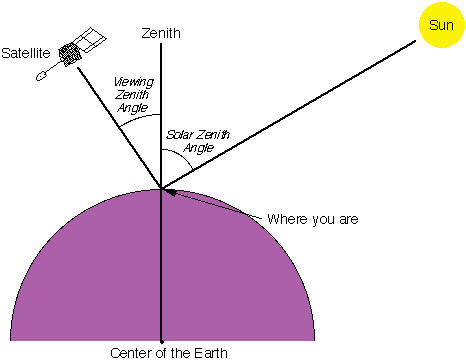
\includegraphics[width=0.6\textwidth]{Figures/ZenithAngles.png}
      \caption{Solar and viewing zenith angles, image copied from \textcite{SZA_Image}, originally from a NASA website.}
      \label{ch_HCHO:fig:zenithangle}
    \end{center}\end{figure}
    
    We use $\nabla I = I_B - I_{B_0}$ to represent the change in intensity due to the absorber. Note that for optically thin absorption, $\nabla I / I_B << 1$, and we can use:
    \begin{equation} \label{Model:omiRecalc:eqn_AMFthin}
    AMF = \frac{\ln{ \left( 1 - \frac{\nabla I}{I_B} \right)} }{\tau_v} \approx \frac{ - \frac{\nabla I}{I_B} }{\tau_v}
    \end{equation}
    $\nabla I$ can also be expressed as the integral of the absorption slices over optical depth increments: 
    \begin{equation*}
      \nabla I = \int_0^{\tau_v}{\frac{\partial I_B}{\partial \tau} \mathrm{d}\tau}
    \end{equation*}
    which can be placed into equation \ref{Model:omiRecalc:eqn_AMFthin}:
    \begin{equation*}
      AMF \approx \frac{-1}{\tau_v} \int_0^{\tau_v}{\frac{\partial \ln{I_B}}{\partial \tau} \mathrm{d}\tau}
    \end{equation*}
    and rewritten as:
    \begin{equation} \label{Model:omiRecalc:eqn_AMFcross}
    AMF = \frac{-1}{\tau_v} \int_0^\infty {\frac{\partial \ln{I_B}}{\partial \tau} \alpha(z)\eta(z)\mathrm{d}z}
    \end{equation}
    where $\alpha(z)$ and $\eta(z)$ represent absorption cross section in m$^2$ molecule$^{-1}$, and number density in molecules m$^{-3}$ respectively. 
    This uses the attenuation cross section relationship to optical depth (see section \ref{Model:Meas:DOAS}).
    
    To represent an average cross section weighted by the absorbing species' vertical distribution, intended to account for temperature and pressure dependence of $\alpha(z)$, $\alpha_e$ is defined as:
    \begin{equation*}
      \alpha_e = \frac{1}{\Omega_v} \int_0^\infty \alpha(z) \eta(z) \mathrm{d}z
    \end{equation*}
    
    This is the same as $ \tau_v = \Omega_v \alpha_e $, which we can place into equation \ref{Model:omiRecalc:eqn_AMFcross} to obtain:
    \begin{equation} \label{Model:omiRecalc:eqn_AMFpreomega}
      AMF=-\int_0^\infty{ \frac{\partial \ln{I_B}}{\partial \tau} \frac{\alpha(z)}{\alpha_e} \frac{\eta(z)}{\Omega_v} \mathrm{d}z }
    \end{equation}
    
    Defining $\omega$(z) as the scattering weights describing the sensitivity of the backscattered spectrum to the abundance of an absorber at altitude z:
    \begin{equation} \label{Model:omiRecalc:eqn_omega}
    \omega(z) = -\frac{1}{AMF_G} \frac{\alpha(z)}{\alpha_e} \frac{\partial \ln{I_B}}{\partial \tau}
    \end{equation}
    It's worth noting that in the OMI satellite product, the provided $\omega(z)$ term does not include the $\frac{1}{AMF_G}$ term and a the calculations which follow therefor do not include this term when utilising the provided $\omega$.
    This is not noted in any of the papers which recalculate the AMF from the OMI product, due to them recalculating the $\omega$ term themselves with a radiative transfer model such as LIDORT.
    
    Plugging equation \ref{Model:omiRecalc:eqn_omega} into equation \ref{Model:omiRecalc:eqn_AMFpreomega} gives us:
    \begin{equation}
      AMF = -\int_0^\infty{ \omega(z) \frac{\eta(z)}{\Omega_v} \mathrm{d}z}
    \end{equation}
    which is best described as the scattering weights ($\omega$) multiplied by the shape factor ($S_z(z) = \frac{\eta(z)}{\Omega_v}$) integrated over altitude z.
    Since we are using the $\omega$ provided by OMI, the AMF$_G$ term is removed from this calculation when compared against \textcite{Palmer2001}.
    
    The integration is done in Python using a simple rectangular method, which multiplies the integrand midpoints by the change in height, and then takes the sum.
    This assumes that the provided scattering weights and shape factors are is linear between the 47 resolved values.
    I recalculate S$_z$(z) using vertical columns of HCHO averaged over 1300-1400~LT from GEOS-Chem.
    As a sanity check I also recalculate S$_\sigma$ and confirm that these shape factors are equivalent, for details see section \ref{Model:omiRecalc:normalising_shapefactor}.
    
    All that remains for recalculating the total vertical column using our new a priori shape factor is to apply the new AMF to the slant columns and grid them onto our chosen resolution.
    Recalculation of the $\omega$ is done seperately, as explained in section \ref{Model:omiRecalc:ppcode}.
    
    
    %TODO: Shape factor plot sigma vs z
    For example see figure TODO: sigma vs z shape factor plot.
    TODO add plot and describe here.
    
    \subsubsection{Normalised vertical shape factor}
      \label{Model:omiRecalc:normalising_shapefactor}
    
      Additionally the vertical shape factor is normalised and the recalculated AMF is checked against that using the non-normalised version.
      The additional steps to calculate a normalised vertical shape factor S$_\sigma$ are first layed out in \textcite{Palmer2001}.
      
      The following equation converts model profile output from ppb into number densities:
      \begin{equation} \label{Model:omiRecalc:eqn_ppb_to_n}
      \eta_{HCHO} = ppb_{HCHO} \times \eta_a \times 10^{-9}
      \end{equation}
      where $\eta_{HCHO}$ is the number density of a HCHO, $\eta_a$ is the number density of air (from model output), and ppb$_{HCHO}$ is the molecules of that species per billion molecules of air.
      In order to normalize these vertical density profiles over the globe, we divide by the modelled total vertical column $\Omega_{HCHO}$ which is determined by:
      \begin{equation*}
      \Omega_{HCHO} = 2.12\times 10^{13} \Sigma_z \left( ppb_{HCHO}(z) (P(z)-P(z+1)) \right)
      \end{equation*}
      where P(z) is the pressure (hPa) at the bottom of altitude level z, the constant 2.12e13 is determined from equation (TODO: Add this equation).
      In effect this equation sums over the molecules per cm$^2$ in each altitude level.
      
      The normalised vertical shape factor S$_z$(z) is defined as:
      \begin{equation} \label{Model:omiRecalc:eqn_ShapeFactor}
      S_z(z) = \frac{\eta(z)}{\Omega_v}
      \end{equation}
      where $\eta(z)$ is the number density in molecules m$^{-3}$.
      
      Now the AMF can be expressed as
      \begin{equation} \label{Model:omiRecalc:eqn_AMFintwSdz}
      AMF = \int_0^\infty \omega(z) S_z(z) \mathrm{d}z
      \end{equation}
      
      
      We have S$_z(z)$ and $\omega(z)$ over the vertical pressure coordinate z at all latitude and longitude points on whatever grid we wish. 
      A conversion to the sigma ($\sigma$) vertical coordinate is performed using $ P = \sigma (P_S - P_T) + P_T$, where $P_T$ is pressure at the top of the atmosphere and $P_S$ is surface pressure.
      In the sigma coordinate system we calculated the shape factor as follows:
      \begin{equation} \label{Model:omiRecalc:eqn_ShapeFactorSigma}
      S_\sigma(\sigma) = \frac{\Omega_a}{\Omega_v}C_{HCHO}(\sigma)
      \end{equation}
      where $\Omega_a$ is the vertical column of air from the surface to the top of the atmosphere and C$_{HCHO}(\sigma)$ is the mixing ratio of HCHO.
      This equation comes from \textcite{Palmer2001}, and is unitless since $\Omega_a / \Omega_v$ is molecules of air per molecule of HCHO; the opposite of $C_{HCHO}$.
    
    \subsubsection{Sigma coordinate conversion}
      \label{Model:omiRecalc:sigmacoord}
      
      Using the vertical coordinate sigma ($\sigma$), which is related to pressure (P) by $P=\sigma \left( P_S - P_T \right) + P_T$, where subscripts S and T represent earth surface and top of the atmosphere respectively.
      The hydrostatic relation $P = - \rho_a g z$, with $\rho_a$, g, being density of air, gravity, respectively lets us switch to the sigma coordinate using:
      \begin{align*}
        \rho_a g z & = \sigma \left( P_S - P_T \right) + P_T \\
        \mathrm{d}\sigma  & = - \frac{ \rho_a g }{ P_S - P_T } \mathrm{d}z
      \end{align*}
      
      Substitution into \ref{Model:omiRecalc:eqn_AMFintwSdz} gives AMF using the sigma coordinates:
      \begin{equation} \label{Model:omiRecalc:eqn_AMFintwSdsigma}
      AMF = \int_0^1 w(\sigma) S_\sigma(\sigma) \mathrm{d}\sigma
      \end{equation}
      Where S$_\sigma$ is defined as a vertical shape factor representing a normalised mixing ratio:
      \begin{equation}
      S_\sigma (\sigma) = \frac{\Omega_a}{\Omega_v}C(\sigma)
      \end{equation}
      where $\Omega_a$ is the vertical column of air and C($\sigma$) is the mixing ratio of the absorber.
      This normalised shape factor is dimensionless.
      This can be useful when running global atmospheric models as the ground altitude is always at $\sigma=1$ and we need not worry about topography. 
    
    
  \subsection{Recalculating the AMF using PP code}
    \label{Model:omiRecalc:ppcode}
    % pp code for AMF recalculation referred to as pp code
    
    Some of the pixels (those covering Australia and most of the zonal band) have their AMFs recalculated using Fortran code written by Paul Palmer, Randal Martin, and updated by Luke Surl.
    I will refer to this as the PP code, and subscript the VCs and AMFs with PP when referring to those calculated through this method.
    This code is computationally expensive, and is only run on pixels within within the region (50-10\degr~S, 160\degr~W-160\degr~E).
    The Fortran code uses a combination of GEOS-Chem a priori profile information and satellite measurement data to calculate the AMF after running the LIDORT radiative transfer calculations to determine scattering.
    The instrument sensitivity or scattering weights, and shape factors for each pixel are calculated which I then integrate vertically to get AMF$_{PP}$s.
    
    
    Code for recalculating AMFs using satellite swaths and modelled aerosol optical depths and gas profiles can be found at \url{http://fizz.phys.dal.ca/~atmos/martin/?page_id=129}. 
    The original method for HCHO is layed out in \textcite{Palmer2001}, with modifications for clouds and use of the LIDORT RTM \parencite{Spurr2002} as described by \textcite{Martin2003}.
    This code does not work as is when using OMI satellite data, and requires modifications performed by Luke Surl at Edinburgh University.
    Additionally the tropopause heights averaged within satellite overpass times output by GEOS-Chem is required, which is achieved by modifying the ND51 diagnostic.
    
    Mie scattering and clouds can complicate the calculation of $\omega$(z), however tables of values for this function at various parameter inputs can be used with modeled vertical shape factors for local AMF calculations.
    This has been done in the PP code and the AMF look-up-table (LUT) can be found in the source code at TODO: add git repo with this code.
    
    First special output is required from GEOS-Chem, averaged between 1300 and 1400 LT, including optical depths at several wavelengths (TODO: list), dust, and HCHO.
    I then pull out a subset of the OMI pixel information into a daily csv file, which can be read by the PP code as modified by Dr. Luke Surl, in conjunction with the GEOS-Chem outputs for each day.
    The PP code then produces a csv of recalculated AMFs which get read by my python code and associated with the corresponding pixel (outlined in \ref{Model:omiRecalc:fig_flow_omhchorp}).
    
  \subsection{Reference sector correction}
    \label{Model:omiRecalc:RSC}
    % where we apply the RSC
    Each satellite slant column measurement is corrected by some amount, based on the divergence from a modeled reference sector.
    HCHO products from OMI and SCIAMACHY both use a median daily remote pacific ocean radiance reference spectrum, over 15$^{\circ}$S-15$^{\circ}$N, 140$^{\circ}$-160$^{\circ}$W where it is assumed that the only significant source of HCHO is methane oxidation \parencite{DeSmedt2008,Barkley2013,Kurosu2014}.
    
    The reference sector correction (RSC) for OMI satellite pixels in this thesis is calculated following \textcite{Abad2016}.
    The RSC is calculated daily and applied to each satellite pixel corresponding to each of the 60 measurement tracks used by OMI, depending also on latitude.
    The reference sector correction is based on the difference between the GEOS-Chem simulated slant columns and OMI slant columns over the meridional band from 140{\degr}W to 160{\degr}W.
    To get the modelled slant columns, each of the AMFs (calculated in prior sections) is applied to the modelled vertical columns using equation \ref{Model:omiRecalc:eqn_AMFratio}.

    % What RSC does
    The RSC method corrects for several problems, however it introduces some a priori model influence.
    One of the problems removed through this correction method is instrument degradation, which can introduce bias over time.
    Another is the possible influence of varying dead/hot pixel masks across 2-D detector arrays such as OMI \parencite{DeSmedt2015}.
    This method also corrects for the errors introduced through correlations between BrO and HCHO absorption cross sections, which are especially significant at high latitudes \parencite{Abad2015}.
    
    % How Vertical columns use reference sector corrections
    Vertical columns in OMI use this oceanic background instead of a solar irradiance spectrum
    In order to recalculate the vertical columns using modelled data, a RSC needs to be applied.
    The correction uses the difference between the slant column ($\Omega_S$) and the reference slant column ($\Omega_{S_0}$) divided by the AMF, plus the modelled reference sector column ($\Omega_{V_B}$):
    \begin{equation*}
      \Omega_{VC} = \frac{ \left( \Omega_S - \Omega_{S_0} \right) }{ AMF } + \Omega_{V_B}
    \end{equation*}
    This method is used in various papers, including \textcite{DeSmedt2008, DeSmedt2012, DeSmedt2015, Barkley2013, Bauwens2016}.
    Recently this correction was expanded (for OMI data) to include latitudinal and instrument track influence by \textcite{Abad2015}.
    
    % How my RSC is defined
    The correction used in this thesis is created based on the difference between the background HCHO measurements from OMI and the GEOS-Chem modelled HCHO columns within the reference sector.
    % Then RSC Longitudinally averaged, binned into 500 lats
    The longitudinal average is taken within the a priori reference sector, as corrections are assumed to be longitudinally invariant.
    The modeled reference sector is interpolated latitudinally to 500 equidistant bins.
    Figure \ref{Model:omiRecalc:RSC:fig_RSCeg} the simulated reference sector VCs as an example, calculated for January 1st 2005.
    In this figure the vertical resolution is increased from 2$^{\circ}$ to 0.36\degr, through linear interpolation, in order to form 500 vertical bins which are used in correcting the satellite data.
    Each day, good satellite measurements taken over the reference sector are used to determine a correction array.
    The correction is based on the difference between measured slant column and the modeled slant column within the reference sector.
    The model does not produce slant columns associated with each measurement, however one is created by multiplying the VC with the associated slant column's AMF.
    
    % This picture was made where?!
    \mypicw{0.7\textwidth}
    {Figures/HCHO/Summary_RSC_Effect8d_20050101.png}
    {%
      Example of remote pacific RSC using 8-day average measurements and one month modelled data.
      $\Omega_{VC}$ shows the uncorrected vertical columns, while $\Omega_{VCC}$ shows the corrected vertical columns.
      OMI corrections shows the correction applied globally based on latitude and OMI track number(sensor).
      $\Omega_{GC}$ shows the GEOS-Chem modelled HCHO VC over the RSC, with $\Omega_{VCC}$ showing the corrected VC over the same area.
    }
    {\label{Model:omiRecalc:RSC:fig_RSCeg}}
    
    % Swath RSC corrections are done 'per track'
    For OMI swaths, each row of measured data contains 60 `Across track'(track) measurements.
    The track index (i) relates a the measurement to one of the 60 columns of data.
    Corrections for each measurement are calculated by taking the difference between the measured slant column and the a priori slant column as follows:
    \begin{equation} \label{Model:omiRecalc:eqn_RSC}
      Correction(i,j) = SC_{HCHO}(i,j) - VC_{GEOS-Chem}(lat(j)) \times {AMF}(i,j)
    \end{equation}
    where j represents a latitude index and $VC_{GEOS-Chem}(lat)$ represents the a priori reference sector vertical column HCHO at the latitude corresponding to j.
    Note that the correction is in molecules cm$^{-2}$.
    % Correction applied over each of the 60 tracks
    The RSC is independently calculated for each of the 60 tracks, at each latitude in the 500 0.36\degr bins.
    This provides a different RSC 
    
    % Interpolated daily RSC to cover missing latitudes
    Due incomplete latitudinal coverage, the correction for each track is interpolated linearly between measurements, with corrections outside of the highest measured latitudes being equal to the corrections at the highest measured latitudes.
    Figure \ref{Model:omiRecalc:RSC:fig_track_correction_interpolations} shows an example of the 60 track corrections for January 1st 2005, the points are satellite measurements and the lines are the interpolations for each track.
    \mypicw{0.7\textwidth}{Figures/HCHO/track_corrections20050101.png}
      {Example of track correction interpolations for January 1st 2005, points represent satellite slant column measurements, with lines interpolating and extrapolating along the latitudinal direction.}
      {\label{Model:omiRecalc:RSC:fig_track_correction_interpolations}}
    
    % Visualisation of RSC refering to plot and 8-day averaged corrections
    Another way to look at this correction is given in the OMI corrections panel of figure \ref{Model:omiRecalc:RSC:fig_RSCeg}, which has the sensors along the x axis, and latitude on the y axis, and shows how for this example 8-day period, the corrections are distributed with more negative values towards the left or right sensors, especially in the tropics.
    
    % One correction per pixel, based on latitude and omi track
    One correction is associated with every good satellite measurement which is used to create a reference sector corrected measurement (Vertical Column Corrected or VCC) through the following equation:
    \begin{equation}
    VCC(i,j) = \frac{SC_{HCHO}(i,j) - Correction(i,lat(j))}{AMF(i,j)}
    \end{equation}
    Finally, for each day, the good satellite measurements are averaged into our own latitude longitude resolution bins along with the associated corrected SC, VC, VCC, AMF, and bin entry count.
    The bin entry count is used to create weighted averages from the daily binned data, which accounts for sparse entries due to filtering.
  
  \subsection{Binning the results daily}
    
    Finally the pixels are binned into a gridded dataset I've called OMHCHORP, as shown in figure \ref{Model:Datasets:OMHCHO:fig_flow_omhchorp}.
    The resolution is chosen to match the native resolution of GEOS-Chem (0.25x0.3125\degr) and the GEOS met data fields.
    %TODO: list of things stored in the daily omhchorp outputs
    Data averaged into this dataset are as follows:
    \begin{enumerate}
      \item satellite SC %($\Omega_{S}$)
      \item satellite AMF %(AMF$_{OMI}$)
      \item satellite VC %($\Omega_{V,OMI}$
      \item satellite RSC VC %($\Omega_{VC,OMI}$)
      \item GEOS-Chem recalculated AMF %(AMF$_{GC}$)
      \item GEOS-Chem recalculated VC %($\Omega_{V,GC}$)
      \item GEOS-Chem recalculated RSC VC %
      \item GEOS-Chem AMF recalculated using Paul Palmer code (AMF$_{PP}$)
      \item GEOS-Chem RSC VC based on AMF$_{PP}$
      \item Smoke AAOD from OMAERUVd (mapped into bins from 1x1\degr resolution)
      \item satellite pixel counts (summed into bins)
      \item fire counts (summed into bins)
    \end{enumerate}
    
    TODO: time per regridding and reprocessing:
    This whole process requires some processing time as well as RAM and computer storage space, and has been performed on the National Computing Infrastructure (NCI) supercomputer cluster.
    In order to reprocess one year of swath files, X GB of daily data was downloaded and then transformed into Y GB of daily gridded data.
    This takes around 90 minutes per day, and is very parallelisable as each day is completely independent once the model has run in each required configuration.
    Initially paralellism was built into the python code, however simply running sending seperate 'jobs' to NCI's process queue was simpler and more scalable.
    As much as possible, processing is done using the HDF-5 format, with some GEOS-Chem output being read and processed from bitpunch to HDF-EOS5 prior to reprocessing.
    The scripts to regrid and reprocess the swath data set are available in the supplementary (TODO).
  
  \subsection{Difference between new and old OMI HCHO columns}
  
    
    Two HCHO products are created, both using GEOS-Chem output at global 2 by 2.5\degr horizontal resolution.
    One uses the OMI product's $\omega_z$ and equation \ref{eqn:AMFintwSdz} in order to calculate an AMF.
    While the other uses code provided by Dr. Paul Palmer, with alterations by Dr. Randal Martin, and Dr. Luke Surl to run LIDORT on the satellite slant columns and the GEOS-Chem output in order to calculate an AMF.
    These two calculations are compared over Australia in figure(s) TODO: Map comparison, regression, and time series once AMFpp is working properly.
    The effect of not recalculating the $\omega_z$ is can be seen in figure \ref{Model:omiRecalc:fig_VCC_pp_fires} which looks at the altered satellite vertical columns using each method.
    
    Figure \ref{Model:omiRecalc:fig_VCC_pp_fires} shows vertical columns of HCHO for: column 1) the original satellite swaths, column 2) recalculated without changing the provided scattering weights, and column 3) fully recalculated vertical columns. 
    Each grid square (at 0.25 by 0.3125\degr lat lon resolution) has been created by binning the recalculated satellite pixels within the month.
    The average pixels per land square is overlaid and changes due to how a fire filter is applied.
    Each row has a stricter fire filter applied from top to bottom, with no fire filter on the first row up to filtering pixels from squares with fires up to 8 days prior.
    This figure looks at March 2005 with biomass burning filtered differently in each row.
    Active fires over the last 0, 1, 2, 4, and 8 days are filtered as the row number increases.
    
    %TODO: figure analysing amf vs amf_gc vs amf_pp
    Figure TODO shows an analysis of the differences between running the recalculation with and without updating the $\omega_z$.
    
    \mypic{Figures/OMI_link/VCC_fires_20050301-20050331.png}{% 
      Column 1: Reference sector corrected HCHO vertical columns $\Omega$ from OMHCHOv003.
      Column 2: $\Omega$ with recalculated a priori shape factors using GEOS-Chem v10.01.
      Column 3: $\Omega$ with recalculated a priori shape factors and scattering weights using GEOS-Chem v10.01 and LIDORT.
      Row 1-5: increasing number of prior days which have active fires are included when masking fire influence.
      }{\label{Model:omiRecalc:fig_VCC_pp_fires}}
    
    TODO: Ask luke if this is true:
    The AMF calculated using Dr. Palmer's code uses a more strict series of filters, leading to fewer satellite based HCHO columns and reduced coverage over Australia.
    Stricter filtering must be balanced against both coverage and the sensitivity of the AMF determination to recalculating $\omega_z$.
  
    Figure TODO: shows global and Australian HCHO averaged total column maps for January 2005, along with the reduced major axis (RMA) regression correlation and percentage difference.
    This comparison shows how reprocessing with an updated model can have a systematic influence on the total column.

\section{Filtering Data}
  \label{Model:Filter}
  
  % Why filter data
  In order to examine only biogenic processes, pyrogenic and anthropogenic influences need to be removed from modelled and measured data.
  As biomass burning can be a large local or transported source of HCHO, CHOCHO, glyoxal, and other compounds we would like to use to determine BVOC emissions, it is advantageous to filter out this source.
  Just filtering active fires does not account for transported smoke plumes, which can carry HCHO precursors.
  One complication when computing HCHO yield from VOC emissions is biomass burning interference, as smoke plumes can contribute to column HCHO.
  In GEOS-Chem we can simply turn off pyrogenic and anthropogenic emissions, however in satellite datasets we need to mask pixels affected by biomass burning.
  
  % How other people have filtered fires
  Influence from biomass burning can be removed through measurements of acetonitrile and CO (eg: \parencite{Wolfe2016, Miller2017}, or else removal of scenes coincident with satellite detected fire counts and aerosol absorption optical depth as done in \textcite{Marais2014}.
  \textcite{Wolfe2016} disregard HCHO measurements when acetonitrile > 210~pptv and CO > 300~ppbv, while acetonitrile > 200~pptv is used to determine fire influence in \textcite{Miller2017}.
  TODO: look at yearly correlation, compare to exponential curve and look for fire outliers
  As seen in TODO: citation, HCHO concentrations scale exponentially with temperature.
  This allows another method for detecting the influence of non-biogenic HCHO emission/creation by looking for outliers above the curve at low temperature.
  \textcite{Zhu2013_poster} has a similar analysis over south-eastern USA showing an exponential correlation of ${HCHO} = \exp(0.15*{T}-9.07)$.
  
  Once the satellite data are quality filtered and gridded, I use additional data to account for anthropogenic and pyrogenic influences, which provides us an estimate of biogenic HCHO.
  MODIS fire counts are used in conjunction with smoke AAOD enhancements (also measured by satellite) to remove data points which may be affected by fires. 
  This has a negative affect on uncertainty, as fewer measurements are available to be averaged.
  This section describes the creation and effects of filters used on satellite data.
  
  
  \subsection{Fire and smoke}
    \label{Model:Filter:fire}
    
    The method used in this thesis follows that of \textcite{Marais2012}, and \textcite{Barkley2013}, with active fires filtered using fire counts, and smoke filtered out using smoke aerosol absorption optical depth (AAOD).
    \textcite{Marais2012} remove pixels colocated with non zero fire counts in any of the prior eight days, within grid squares with 1 x 1\degr resolution.
    \textcite{Barkley2013} use fires from the preceding and concurrent day, within local or adjacent grid squares, with grid resolution of 0.25 x 0.3125\degr.
    We use the MODIS fire counts, detected from space using the combined product from Terra and Aqua (Terra at 10:30, 22:30 LT; Aqua at 13:30, 01:30 LT).
    Smoke plumes can be filtered using product OMAERUVd, although care needs to be taken when deciding the threshhold for smoke detection \parencite{Marais2012}.
    
    % My method for fire filtering:
    When analysing satellite OMHCHO vertical columns ($\Omega$), the following steps are performed in order to mask influence from biomass burning:
    \begin{enumerate}
      \item MOD14A1 daily gridded Aqua/Terra combined fire counts are read at 1x1~km$^2$ resolution, and binned into 0.25x0.3125\degr bins, matching the resolution of binned $\Omega$.
      \item A rolling mask is formed which removes $\Omega$ if one or more fires are detected in a grid square, or in the adjacent grid square, up to 2 days previously.
      This includes the 'current' day, making 3 days of fires in total being filtered out on each day.
      % TODO AAOD filtering description
      \item AAOD at 500~nm is mapped from OMAERUVd 1x1\degr resolution onto the 0.25x0.3125\degr resolution.
      \item An AAOD threshold of 0.03 is determined through visual analysis of AAOD distributions over several days, including days with and without influence from active fires, dust, and transported smoke plumes.
      \item Grid squares with AAOD over this threshhold are considered potentially affected by transported fire smoke.
    \end{enumerate}
  
    % Smoke AAOD determination:
    Determining the AAOD due to smoke can be difficult since both smoke and dust absorb UV radiation \parencite{Ahn2008,Marais2012}.
    AAOD is should be less sensitive to cloud contamination than AOD, and I use AAOD from the daily gridded level 3 satellite product OMAERUVd \parencite{Ahn2008} described in section \ref{Model:Datasets:OMAERUVd} to provide a filter for smoke plumes.
    Although removing gridsquares with dust reduces how much data is available to analyse, it's considered a minor problem as dust in Australia is highly episodic and should not affect more than a few days per year, especially over regions with high tree coverage \parencite{Shao2007}.
    
    Filtering fire smoke using AAOD is done by removing OMHCHO gridsquares where the AAOD is above a 0.03, after the AAOD is mapped from 1x1\degr to the same 0.25x0.3125\degr resolution as our OMHCHO gridded product.
    The threshhold is determined through analysing AAOD over Australia in 4 scenarios: normal conditions, active local fires, during influence from transported fire smoke, and large scale dust storms.
    Figure \ref{Model:Filter:fire:fig_typicalAAOD} shows AAOD (columns 1 and 2), with AAOD distribution in column 3, along with satellite imagery on the same day in column 4 (from \url{https://worldview.earthdata.nasa.gov/}).
    The scenarios listed are shown from row 1 to 4, and AAOD $=$ 0.03 is demarked by a horizontal line in the density plots in column 3.
    
    \mypic{Figures/OMI_link/typical_AAODs.png}
      {AAOD from OMAERUVd (columns 1, 2, 3) over Australia for four different scenarios (rows 1-4). Scenes from the same day are taken from the EOS Worldview website \url{https://worldview.earthdata.nasa.gov/}.}
      {\label{Model:Filter:fire:fig_typicalAAOD}}
  
  % TODO: Quick analysis of how much data is lost with smoke filtering?
  
    \subsubsection{Checking that fire masks are influencing pyrogenic HCHO}
      
      Looking at temperature can provide evidence of pyrogenic HCHO.
      HCHO precursors are heavily tied to temperature (TODO:cite), and model output shows how higher temperature leads to an increase in HCHO levels.
      Figures \ref{Model:Analysis:HCHO:fig_hcho_vs_temp_SEA_200501} - \ref{Model:Analysis:HCHO:fig_hcho_vs_temp_SWA_200501} show the relationship between temperature and HCHO, for January 2005, within subsets of Australia.
      A reduced major axis regression is used to determine the correlation between surface temperature (X axis) and HCHO (Y axis)..
      Using the natural log of HCHO we can take the linear regression and then exponentiate each side in the equation $\ln{Y} = m{X}+b$ to get ${Y} = \exp{m{X}+b}$. 
      This gives us the exponential fit as shown, with the correlation coefficient between $\ln{HCHO}$ and temperature.
      The distributions of exponential correlation coefficients and exponential 'm' terms is shown in the embedded plot, with one datapoint available for each grid square where the regression is performed.
      
      When applying the fire mask to the modelled HCHO, we can analyse how this affects the relationship to temperature.
      One cause of high HCHO at lower temperatures (above the exponential regression line) can be emissions from fires.
      If we see these datapoints affected by the firemask then this suggests that the mask is working correctly.
      TODO plot showing how fire mask affects HCHO - Temperature relationship
      
      
      \begin{figure}
        \includegraphics[width=\textwidth]{Figures/OMI_link/GC/HCHO_vs_temp_SEA_20050101-20050228.png}
        \caption{%
          Top panel: surface temperature averaged over January and February 2005.
          Bottom panel: surface temperature correlated against temperature over, with different colours for each gridbox, and the combined correlation. 
          A reduced major axis regression is used within each gridbox (shown in top panel) using daily overpass time surface temperature and HCHO amounts (ppbv).
          The distribution of slopes and regression correlation coefficients (one datapoint per gridbox) for the exponential regression is shown in the embedded plot.
          }
        \label{Model:Analysis:HCHO:fig_hcho_vs_temp_SEA_200501}
        \end{figure}
          
        \begin{figure}
          \includegraphics[width=\textwidth]{Figures/OMI_link/GC/HCHO_vs_temp_NA_20050101-20050228.png}
          \caption{%
            As figure \ref{Model:Analysis:HCHO:fig_hcho_vs_temp_SEA_200501} but for northern Australia.
            }
          \label{Model:Analysis:HCHO:fig_hcho_vs_temp_NA_200501}
        \end{figure}
          
        \begin{figure}
          \includegraphics[width=\textwidth]{Figures/OMI_link/GC/HCHO_vs_temp_SWA_20050101-20050228.png}
          \caption{%
            As figure \ref{Model:Analysis:HCHO:fig_hcho_vs_temp_SEA_200501} but for south-western Australia.
            }
          \label{Model:Analysis:HCHO:fig_hcho_vs_temp_SWA_200501}
        \end{figure}
  
  \subsection{NOx}
    \label{Model:Filter:NOx}
    
    % Why filter high NO? Anthro influence
    Enhanced NO$_2$ concentrations can indicate anthropogenic influence over Australia.
    In order to filter out these influences on satellite HCHO measurements, a filter is designed using the OMNO2d product which includes tropospheric NO$_2$ columns.
    
    % Nox analysis from OMNO2d
    OMNO2d from 2005 is used to determine a suitable threshhold for anthropogenic influence by looking at NO$_2$ columns near several major cities in the south eastern sector of Australia.
    The mean, standard deviation, and time series over Australia of tropospheric NO$_2$ seen by Aura is shown in figure \ref{Model:Filter:NOx:fig_omno2_timeseries}.
    The average tropospheric NO$_2$ column for averaged within all of Australia and then each region shown in this figure is listed in table TODO \ref{Model:Filter:NOx:tab_summary}.
    
    \mypic{Figures/OMI_link/OMNO2_timeseries_2005.png}
    {Mean (top left) and standard deviation (top right) of OMNO2d daily 0.25x0.25\degr tropospheric cloud filtered NO$_2$ columns. Time series for Australia, and each region (by colour) shown in the bottom panel, with mean for that region shown on the right. A grey shaded area depicts the 25th to 75th percentiles of Australia averaged NO$_2$ columns for each day in the time series, with a thicker black line showing the Australia-wide mean value.}
    {\label{Model:Filter:NOx:fig_omno2_timeseries}}
    
    % Filters and Threshhold determination and reasoning
    Anthropogenic influences on the NO$_2$ columns are clearly visible near major cities in Australia.
    A filter is created each year from the OMNO2d product in two steps:
    \begin{enumerate}
      \item Daily gridsquares with NO$_2$ greater than 10$^{15}$\moleccm  are flagged as anthropogenic.
      \item After taking the yearly average over Australia, any gridsquares greater than $1.5 \times 10^{15}$\moleccm are flagged for the whole year.
    \end{enumerate}
    This removes both the gridsquares close enough to cities to be affected by their emissions year round, as well as effects from transported pollution plumes.
    The affects of applying this filter to the OMNO2d product itself can be seen in figure \ref{Model:Filter:NOx:fig_omno2_threshaffect}
    
    \mypic{Figures/OMI_link/OMNO2_threshaffect_2005.png}
    {2005 OMNO2d NO$_2$ column mean before (left) and after (right) applying the threshhold filters as described in the text. Time series for Australia, and each region (by colour) shown in the bottom panel, with mean for that region shown on the right.}
    {\label{Model:Filter:NOx:fig_omno2_threshaffect}}
    
    % Threshhold analysis
    The same regions as in figure \ref{Model:Filter:NOx:fig_omno2_timeseries} are shown again in figure \ref{Model:Filter:NOx:fig_omno2_densities}, with NO$_2$ pixels densities for each region shown, along with the threshold of $1 \times 10^{15}$\moleccm.
    This led to a reduction of TODO gridsquares from the total available measurement space over Australia.
    The removal of gridsquares which went above the yearly averaged limit of 1.5e15\moleccm further reduced the available data by TODO gridsquares.
    
    \mypic{Figures/OMI_link/OMNO2_densities_2005.png}
    {2005 OMNO2d NO$_2$ column means (top left), along with column amount distributions for Australia (top right) and each region shown in the area map (by colour)}
    {\label{Model:Filter:NOx:fig_omno2_densities}}
    
    \begin{table}
      \caption{NO$_2$ averages by region before and after filtering for anthropogenic emissions using 2005 data from the OMNO2d product.}
      \begin{tabular}{ c c c c }
        \hline
        \textbf{Region} & \textbf{NO$_2$} & \textbf{NO$_2$ after filtering} & \textbf{\% Data lost} 
        \\ \hline
        Aus & 1 & 2 & 3 \\
        BG & 1 & 2 & 3 \\
        Syd & 1 & 2 & 3 \\
        Melb & 1 & 2 & 3 \\
        Adel & 1 & 2 & 3 \\
        \hline
      \end{tabular}
      \label{Model:Filter:NOx:tab_summary}
    \end{table}
    
    % Affects of filtering
    % TODO: tabulate or summarise no2 filtering
    
    \subsection{Summary of filters effects on HCHO}
      
     
\section{Data Access}
TODO: ADD MORE HERE
\label{Model:DataAccess}
\begin{description}
  \item[OMNO2d] Daily satellite NO$_2$ product downloaded from \url{https://search.earthdata.nasa.gov/search}, DOI:10.5067/Aura/OMI/DATA3007. 
  See more information in section %TODO:
  
  \item[SPEI] Monthly standardised precipitation evapotranspiration index (metric to determine drought stress) downloaded from \url{http://hdl.handle.net/10261/153475} with DOI:10.20350/digitalCSIC/8508.
  See more information in section %TODO:
  
  \item[OMHCHO] Satellite swaths of HCHO slant columns downloaded from TODO, with DOI TODO
  
\end{description}